重力波とは, 一般相対性理論から導かれる時空の歪みが波として光速で伝播する現象である. 重力波は, 非常に強い透過力を持っており, 新しい観測手段として宇宙物理学を進歩させることができると期待されている. \\
\quad この章では重力波の導出や性質, および主な波源について述べた後, レーザー干渉計型重力波検出器について記す. 
\section{重力波}
\subsection{重力波の導出}
\renewcommand{\thefootnote}{\arabic{footnote}}
一般相対性理論では4次元Riemann時空を用いて時間(1次元)と空間(3次元)を表す. この時空において, 無限に近接する2点間の距離は計量テンソル$g_{\mu\nu}$を用いて
\begin{equation}
{\rm d}s^{2}=g_{\mu\nu}{\rm d}x^{\mu}{\rm d}x^{\nu}\qquad(\mu,\nu=0,1,2,3),
\label{eq2.1}
\end{equation}
と定義される. ここで$x^0$は時間座標, $x^i\quad(i=1,2,3)$は空間座標を表す. なお, 本論文ではこれ以降, ギリシャ文字の添字が0,1,2,3, ローマ文字の添字が1,2,3を表すものとする. 式(\ref{eq2.1})より, 計量テンソル$g_{\mu\nu}$は対称テンソルであり, 一般相対論における時空の性質(重力場の性質)を表すことが分かる. \\
\quad 一方, 時空上のある点で局所Lorentz系をとった時, その点において時空は平坦であり, Minkowski時空と呼ばれる. また, その時空の計量は
\begin{equation}
g_{\mu\nu}=\eta_{\mu\nu}\equiv
\begin{pmatrix}
-1 &   &   &  \\
   & 1 &   &  \\
   &   & 1 &  \\
   &   &   & 1\\
\end{pmatrix},
\label{eq2.2}
\end{equation}
と表される. \\
\quad さて, 重力場を含む時空はEinstein方程式
\begin{equation}
G_{\mu\nu}\equiv R_{\mu\nu}-\frac{1}{2}g_{\mu\nu}R=\frac{8\pi G}{c^4}T_{\mu\nu},
\label{eq2.3}
\end{equation}
で記述される. \\
\quad ここで$G_{\mu\nu}$はEinsteinテンソル, $R_{\mu\nu}$はRicchiテンソル, $G$は重力定数, $c$は光速, $T_{\mu\nu}$はエネルギー運動量テンソルである. なお, 
\begin{equation}
\Gamma^{\rho}_{\mu\nu}=\frac{1}{2}g^{\mu\nu}(\partial_{\rho}g_{\sigma\nu}+\partial_{\sigma}g_{\rho\nu}-\partial_{\nu}g_{\rho\sigma}),
\end{equation}
\begin{equation}
R^{\alpha}_{\mu\rho\nu}=\partial_{\rho}\Gamma^{\alpha}_{\mu\nu}-\partial_{\nu}\Gamma^{\alpha}_{\mu\rho}+\Gamma^{\alpha}_{\sigma\rho}\Gamma^{\sigma}_{\mu\nu}-\Gamma^{\alpha}_{\sigma\nu}\Gamma^{\sigma}_{\mu\rho},
\end{equation}
\begin{equation}
R_{\mu\nu}=R^{\alpha}_{\mu\alpha\nu},
\end{equation}
\begin{equation}
R=g^{\mu\nu}R_{\mu\nu},
\end{equation}
である($\Gamma^{\rho}_{\mu\nu}$はChristoffel記号, $R^{\alpha}_{\mu\rho\nu}$はRiemannテンソル, $R$はRicchiスカラー). つまりEinstein方程式(\ref{eq2.3})の左辺が時空の性質, 右辺が物質場を表している. よってEinstein方程式は, 質量-エネルギー分布が時空の歪みを作り出しと解釈することができ, さらに物質の変動が重力場の変動をもたらすことも示している. \\
\quad Einsteinは, 平坦な時空に微小な線形摂動が存在する弱い重力場を考えることで重力波を導いた. この微小線形摂動を$h_{\mu\nu}$とすると, 摂動を含む計量はMinkowski計量(\ref{eq2.2})を用いて
\begin{equation}
g_{\mu\nu}=\eta_{\mu\nu}+h_{\mu\nu},
\end{equation}
と書き表される. 以下ではこのように線形下された一般相対性理論において, 重力波を導出する. \\
はじめに
\begin{equation}
h\equiv\eta^{\mu\nu}h_{\mu\nu},
\end{equation}
\begin{equation}
\bar{h}_{\mu\nu}\equiv h_{\mu\nu}-\frac{1}{2}\eta_{\mu\nu}h,
\end{equation}
を定義する. ここで, 
\begin{equation}
\bar{h}_{\mu\nu}\equiv\eta^{\mu\nu}=h-2h=-h,
\end{equation}
であることから, 
\begin{equation}
h_{\mu\nu}=\bar{h}_{\mu\nu}-\frac{1}{2}\eta_{\mu\nu}\bar{h},
\end{equation}
となる. また, ダランベール演算子$\Box\equiv\eta_{\mu\nu}\partial^{\mu}\partial^{\nu}=\partial_{\mu}\partial^{\mu}$を用いるとRicchiテンソルおよびRicchiスカラーは
\begin{equation}
R_{\mu\nu}=-\frac{1}{2}\left(\Box\bar{h}_{\mu\nu}-\partial^{\alpha}\partial_{\mu}\bar{h}_{\alpha\nu}-\partial^{\alpha}\partial_{\nu}\bar{h}_{\alpha\mu}-\frac{1}{2}\eta_{\mu\nu}\Box\bar{h}\right),
\end{equation}
\begin{equation}
R=-\frac{1}{2}\left(-\Box\bar{h}-2\partial^{\alpha}\partial^{\mu}\bar{h}_{\alpha\mu}\right),
\end{equation}
となる. これよりEinstein方程式(\ref{eq2.3})の左辺は
\begin{equation}
-\frac{1}{2}\left(\Box\bar{h}_{\mu\nu}+\eta_{\mu\nu}\partial^{\alpha}\partial^{\beta}\bar{h}_{\alpha\beta}-\partial^{\alpha}\partial_{\nu}\bar{h}_{\mu\alpha}-\partial^{\alpha}\partial_{\mu}\bar{h}_{\nu\alpha}\right),
\end{equation}
となるので, 式(\ref{eq2.3})を書き直すと
\begin{equation}
\Box\bar{h}_{\mu\nu}+\eta_{\mu\nu}\partial^{\alpha}\partial^{\beta}\bar{h}_{\alpha\beta}-\partial^{\alpha}\partial_{\nu}\bar{h}_{\mu\alpha}-\partial^{\alpha}\partial_{\mu}\bar{h}_{\nu\alpha}=-\frac{16\pi G}{c^4}T_{\mu\nu},
\end{equation}
ここで真空の場合 ($T_{\mu\nu}=0$) を考え, さらにLorenzゲージ条件
\begin{equation}
\frac{\partial \bar{h}^{\mu}_{\nu}}{\partial x_{\nu}}=0,
\label{eq2.17}
\end{equation}
を課す\footnote{Lorenzゲージ条件は以下に示す通り, 常に課すことができる. \\座標変換$x^{\mu}\rightarrow x^{\prime\mu}=x^{\mu}+\xi^{\mu}(x)$に対して
\begin{equation*}
\bar{h}_{\mu\nu}(x)\rightarrow\bar{h}^{\prime}_{\mu\nu}(x^{\prime})=\bar{h}_{\mu\nu}(x)-\partial_{\mu}\xi_{\nu}(x)-\partial_{nu}\xi_{\mu}(x)+\eta_{\mu\nu}\partial_{\alpha}\xi^{\alpha}(x),
\end{equation*}
となる. また, 
\begin{equation*}
\partial^{\nu}\bar{h}_{\mu\nu}(x)\rightarrow(\partial^{\nu}\bar{h}_{\mu\nu})^{\prime}(x^{\prime})=\partial^{\nu}\bar{h}_{\mu\nu}(x)-\Box\xi_{\mu}(x),
\end{equation*}
なので
\begin{equation*}
\Box\xi_{\mu}(x)=\partial^{\nu}\bar{h}_{\mu\nu}(x),
\tag{A}
\end{equation*}
となる$\xi$が常に存在すれば良いことが分かる. ここで, ある関数$f_{\mu}(x)$を用いて$\partial^{\nu}\bar{h}_{\mu\nu}(x)=f_{\mu}(x)$と書くと
\begin{equation*}
\Box\xi_{\mu}(x)=f_{\mu}(x),
\end{equation*}
となる. この式の解は
\begin{equation*}
\Box G(x-y)=\delta^{4}(x-y),
\end{equation*}
を満たすGreen関数$G(x)$を用いて
\begin{equation*}
\xi_{\mu}(x)=\int{\rm d}^4yG(x-y)f_{\mu}(y),
\end{equation*}
と書ける. よって式(A)の解は常に存在し, Lorenz条件は常に課しても良いことが分かる. 
}. すると線形化されたEinstein方程式は
\begin{equation}
\Box\bar{h}_{\mu\nu}=0,
\label{eq2.18}
\end{equation}
となる. これが線形化された一般相対性理論における重力場の振る舞いを記述する式である. \\
\subsection{重力波の伝播}
式(\ref{eq2.18})は平面波解を持ち, 計量の揺らぎ$\bar{h}_{\mu\nu}$が光速で伝播することを表す. この平面波解が重力波である. 以下では重力波の伝播とその性質について考える. \\
\quad 式(\ref{eq2.17})のLorenz条件はゲージを完全に決めていない. そのため, Lorenz条件を満たす座標系$x^{\mu}$に対し, 
\begin{equation}
x^{\mu}\rightarrow x^{\prime\mu}=x^{\mu}+\xi^{\mu},
\end{equation}
\begin{equation}
\Box\xi_{\mu}=0,
\label{eq2.20}
\end{equation}
のような変換を考えてもLorenz条件は破られない. ここで, 平坦な時空の場合$\Box$と$\partial_{\mu}$が可換であることを考えると
\begin{equation}
\xi_{\mu\nu}\equiv\partial_{\mu}\xi_{\nu}+\partial_{\nu}\xi_{\mu}-\eta_{\mu\nu}\partial_{\alpha}^{\alpha},
\end{equation}
に対して$\Box\xi_{\mu\nu}=0$が成り立つことが分かる. よって式(\ref{eq2.20})を用いてゲージ自由度を固定すると$\bar{h}_{\mu\nu}$の自由度を4つ減らすことができる. つまり, Lorenz条件の4式および式(\ref{eq2.20})の4式で$\bar{h}_{\mu\nu}$の自由度は2つとなる. \\
\quad 次に, その2つの自由度で$\bar{h}_{\mu\nu}$を書き表す. トレースが$\bar{h}=0$となるように$\xi^{0}$を, また$h^{0i}(x)=0$となるように$\xi^i(x)$を選ぶ. このとき$\bar{h}_{\mu\nu}=h_{\mu\nu}$であるから, Lorenz条件において$\mu=0$とおいた式
\begin{equation}
\partial^0h_{00}+\partial^{i}h_{0i}=0,
\end{equation}
より, 
\begin{equation}
\partial^{0}h_{00}=0\quad (\because h_{0i}=0),
\end{equation}
となる. つまりNewtonポテンシャルに相当する成分である$h_{00}$は時間に依らないことが分かる. しかし, 伝播する重力波を扱っているのでこの成分は関係なく, $h_{00}=0$としてよい. 以上をまとめると
\begin{equation}
\begin{split}
h^{0\mu}=0\\
{h^i}_i=0\\
\partial^jh_{ij}=0,\\
\end{split}
\label{eq2.24}
\end{equation}
であり, これをTT (Transverse-Traceless) ゲージ\footnote{3つ目の式$\partial^jh_{ij}=0$から重力波は横波 (Transverse) であり, 2番目の式${h^i}_i=0$からトレースが0である (Traceless) ことが分かる. }と呼ぶ\cite{19}. 以下ではTTゲージ下での計量を$h_{ij}^{\rm TT}$と記す. \\
\quad さて, 線形化されたEinstein方程式(\ref{eq2.17})は平面波解
\begin{equation}
h_{ij}^{\rm TT}(x)=e_{ij}({\bf k})e^{ikx},
\end{equation}
を持つ. ただし, $kx=k^{\mu}x_{\mu}$であり, $k^{\mu}=(\omega_{\rm GW}/c,{\bf k})$, $\omega_{\rm GW}/c=\left|{\bf k}\right|$である. なお, $e_{ij}({\bf k})$は偏極テンソル, $\omega_{\rm GW}$は重力波の周波数である. このとき波数ベクトル${\bf k}$で記述される単色平面波を考えると, 式(\ref{eq2.24})より$h_{ij}^{\rm TT}$の0でない要素は重力波の進行方向${\bf n}={\bf k}/\left|{\bf k}\right|$と直交する. \\
\quad ここで, 重力波が$z$軸($x^{3}$軸)に進むとする(${\bf n}$を$z$軸に沿うように選ぶ)と, 式(\ref{eq2.24})と$h_{ij}^{\rm TT}$の対称性より
\begin{equation}
h_{ij}^{\rm TT}(t,z)=
\begin{pmatrix}
h_{+} & h_{\times} & 0 \\
h_{\times} & -h_{+} & 0 \\
0 & 0 & 0
\end{pmatrix}
\cos\left[\omega_{\rm GW}(t-z/c)\right],
\end{equation}
となる. ただし, $h_{+},h_{\times}$は2つの独立な偏極モードを表す. さらに, $h_{+}(t)=h_{+}\cos\left[\omega_{\rm GW}(t-z/c)\right]$, $h_{\times}(t)=h_{\times}\cos\left[\omega_{\rm GW}(t-z/c)\right]$とすると
\begin{equation}
h_{ab}^{\rm TT}(t,z)=
\begin{pmatrix}
h_{+}(t) & h_{\times}(t) \\
h_{\times}(t) & -h_{+}(t)
\end{pmatrix}
_{ab}\qquad (a,b=1,2),
\label{eq2.27}
\end{equation}
と書ける. \\
\quad 今, $x$軸($x^{1}$軸)方向に沿って$\epsilon$だけ離れた2つの自由質点を考える. このとき, 式(\ref{eq2.27})で表される$z$軸方向の重力波の影響はこれらの質点の固有距離を考えることで分かる. 質点がはじめ静止していたとすると, 固有距離$\Delta l$は
\begin{equation}
\Delta l\equiv\int\left|{\rm d}s^2\right|^{1/2}=\int_0^{\epsilon}\left|g_{11}\right|^{1/2}{\rm d}x^1\simeq\left|g_{11}\right|^{1/2}\epsilon\simeq\left(1+\frac{1}{2}h_{11}\right)\epsilon,
\end{equation}
これより重力波は自由質点間の距離を変化させることが分かる. \\
\quad 次に, 固有距離$\epsilon^i=(\epsilon^x,\epsilon^y,\epsilon^z)$だけ離れた2質点に$z$軸方向に進む重力波が入射したとする. このとき式(\ref{eq2.27})に従う重力波を仮定すると, この固有距離は
\begin{equation}
\frac{1}{2}
\begin{pmatrix}
h_{+}(t) & h_{\times}(t) \\
h_{\times}(t) & -h_{+}(t) \\
\end{pmatrix}
\begin{pmatrix}
\epsilon^x \\
\epsilon^y \\
\end{pmatrix}
=\frac{1}{2}h_{+}(t)
\begin{pmatrix}
\epsilon^x \\
-\epsilon^y \\
\end{pmatrix}
+\frac{1}{2}h_{\times}(t)
\begin{pmatrix}
\epsilon^y \\
\epsilon^x \\
\end{pmatrix},
\end{equation}
と計算される. これより偏極モードについて, \\
\qquad 1) $h_{+}$モード(plus mode)は$x$軸に伸ばすと共に, $y$軸方向には縮める\\
\qquad 2) $h_{\times}$モード(cross mode)は$h_{+}$を45度回転させたものである\\
ということが言える. これを表したものが図\ref{fig2.1}であり, 重力波が到来したとき, 質点は潮汐的な運動をすることが分かる. 
\begin{figure}[H]
\begin{center}
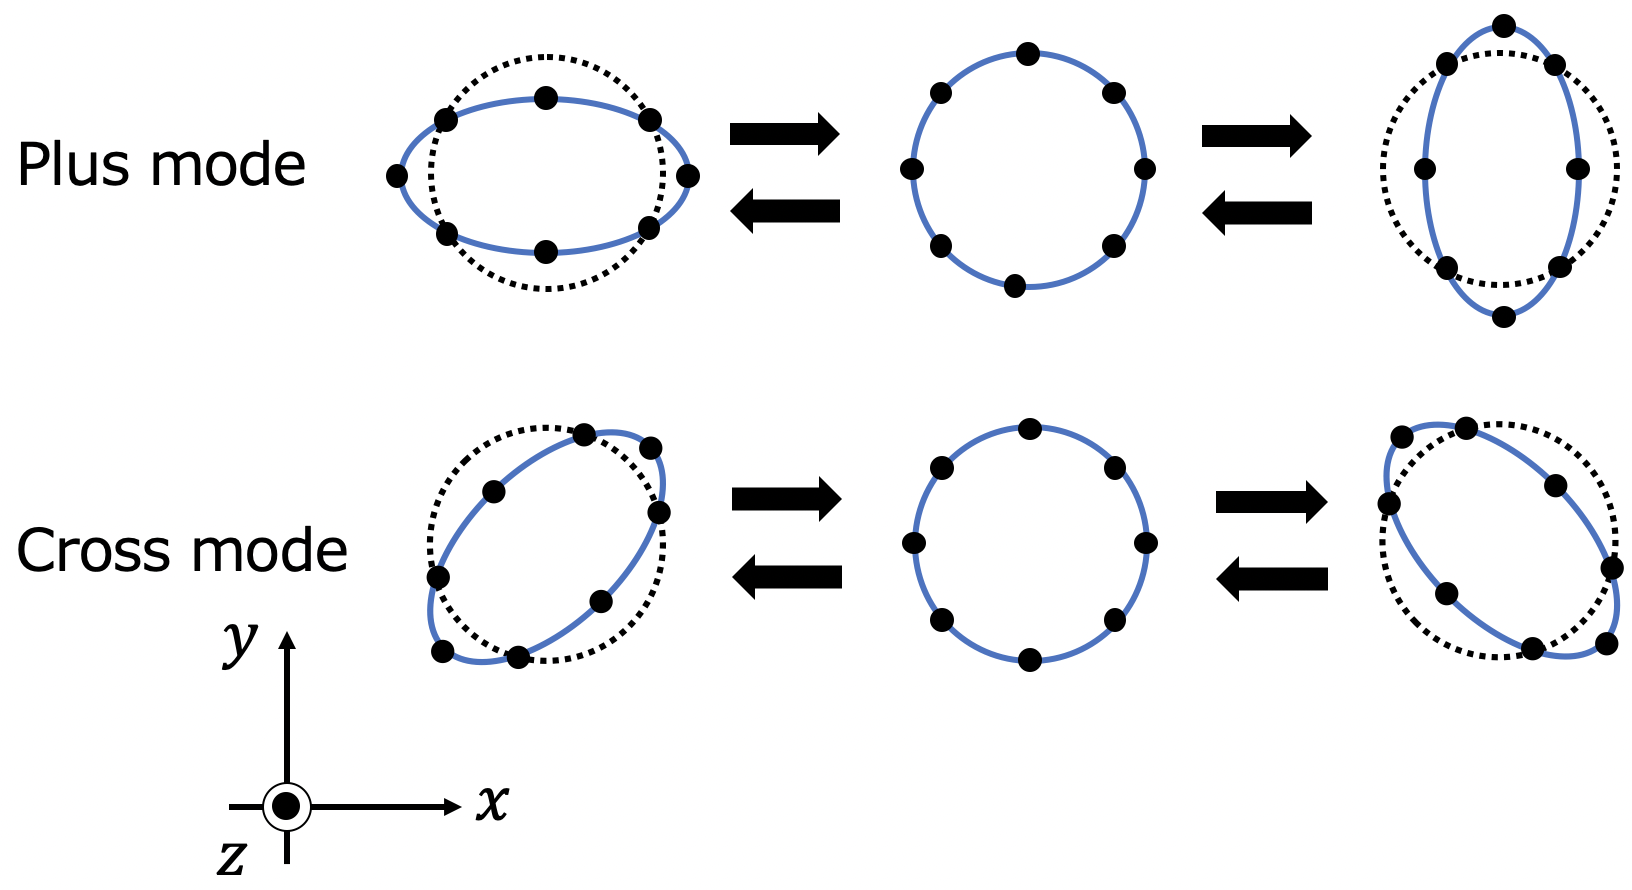
\includegraphics[width=140mm]{fig2_1.png}
\caption[重力波の偏光モード]{重力波の偏光モードの模式図. 重力波の入射によって, 質点間の固有距離が中央の初期状態から潮汐的に運動する様子を表している}
\label{fig2.1}
\end{center}
\end{figure}
\subsection{重力波の輻射}
電磁波の輻射から類推すると, 重力波は加速度をもった質量によって生まれることが分かる. しかし, 重力波では双極子放射が存在しない(質量は常に正であるから, 双極子モーメントが存在しない)ので, 4重極子モーメント(あるいはそれ以上の多重極)からの輻射を考えるという違いがある. \\
\quad エネルギー運動量テンソルが存在する場合, (\ref{eq2.18})式は
\begin{equation}
\Box\bar{h}_{\mu\nu}=\left(-\frac{1}{c^2}\frac{\partial^2}{\partial t^2}+\frac{\partial^2}{\partial x_i^2}\right)\bar{h}_{\mu\nu}=-\frac{16\pi G}{c^4}T_{\mu\nu},
\label{eq2.30}
\end{equation}
となる. また, Green関数$G(\bm{x}-\bm{x}^{\prime})$を
\begin{equation}
G(\bm{x}-\bm{x}^{\prime})=\frac{1}{4\pi\left|\bm{x}-\bm{x}^{\prime}\right|}\delta(x^0_{\rm ret}-x^{\prime0})
\end{equation}
\begin{equation}
x_{\rm ret}^0\equiv ct_{\rm ret},\quad t_{\rm ret}=t-\frac{\left|\bm{x}-\bm{x}^{\prime}\right|}{c},
\end{equation}
と書くと式(\ref{eq2.30})の解として
\begin{equation}
\bar{h}_{\mu\nu}(x^0,\bm{x})=\frac{4G}{c^4}\int\frac{T_{\mu\nu}\left(x^0-\frac{\left|\bm{x}-\bm{x}^{\prime}\right|}{c},\bm{x}^{\prime}\right)}{\bm{x}-\bm{x}^{\prime}}{\rm d}\bm{x}^{\prime},
\label{eq2.33}
\end{equation}
を得る. 真空でない($T_{\mu\nu}\neq0$)範囲が十分小さく, 観測者が波源から十分離れているとすると式(\ref{eq2.33})は多重極展開の最低次の項として, 
\begin{equation}
\bar{h}_{ij}(t,\bm{x})=\frac{1}{r}\frac{2G}{c^4}\ddot{Q}_{ij}(t^{\prime}),
\label{eq2.34}
\end{equation}
となる. ただし, $r\equiv\left|\bm{x}-\bm{x}^{\prime}\right|$,$t^{\prime}\equiv t-r/c$であり, $Q_{ij}$は四重極モーメント
\begin{equation}
Q_{ij}(t^{\prime})=\int\rho(t^{\prime},\bm{x})\left(x_{i}^{\prime}x_{j}^{\prime}-\frac{1}{3}\delta_{ij}x^{i\prime}x^{j\prime}\right)d\bm{x}^{\prime},
\end{equation}
である.  \\
\quad また, Larmorの公式から類推すると, この時の重力波の光度は
\begin{equation}
\mathcal{L}_{\rm gw}=\frac{G}{5c^5}\left<\left(\dddot{Q}_{ij}\right)^2\right>,
\label{eq2.36}
\end{equation}
となる. ここで, 系の特徴的な質量$M$, サイズ$R$, 時間スケール$T$, 速度$v$を考えると四重極モーメントの時間3階微分は
\begin{equation}
\dddot{Q}_{ij}\sim\frac{MR^2}{T^3}\sim\frac{Mv^3}{R},
\end{equation}
と近似できる. これより光度(\ref{eq2.36})のオーダーを計算すると
\begin{equation}
\mathcal{L}_{\rm GW}\sim\frac{G}{c^5}\left(\frac{M}{R}\right)^2v^6\sim3.6\times10^{59}\,\,[{\rm erg}/{\rm s}]\left(\frac{r_{\rm sch}}{R}\right)^2\left(\frac{v}{c}\right)^6,
\end{equation}
となる($r_{\rm sch}=2GM/c^2$はSchwarzschild半径). このエネルギー放射率は極めて小さく, 地球上に重力波源を作るのは難しいので天体からの放射に期待しているのである. ここで天体は普通, 自己重力に束縛されているので運動エネルギーと位置エネルギーの間に関係がある(virial定理)と仮定でき, 
\begin{equation}
Mv^2\sim\frac{GM^2}{R}.
\end{equation}
これを用いると式(\ref{eq2.36})は
\begin{equation}
\mathcal{L}_{\rm GW}\sim3.6\times10^{59}\,\,[{\rm erg}/{\rm s}]\left(\frac{r_{\rm sch}}{R}\right)^5,
\end{equation}
となる. これより, コンパクト天体(ブラックホールや中性子星など)が重力波源の候補になることが分かる. \\
さらに, 輻射された重力波の振幅を考えるために式(\ref{eq2.34})に対して
\begin{equation}
h\sim\frac{1}{r}\frac{2G}{c^4}\frac{\partial^2}{\partial t^2}(MR^2)\sim\frac{1}{r}\frac{2GMv^2}{c^4}\sim\frac{r_{\rm sch}}{r}\left(\frac{v}{c}\right)^2,
\label{eq2.41}
\end{equation}
という近似を行う. また, 重力波によるエネルギー放射効率を$\epsilon$として
\begin{equation}
\epsilon\sim\left(\frac{r_{\rm sch}}{R}\right),
\end{equation}
とパラメタ化すると式(\ref{eq2.41})は
\begin{equation}
h\sim\epsilon^{2/7}\frac{r_{\rm sch}}{2r}\sim1.5\times10^{-18}\left(\frac{\epsilon}{0.1}\right)^{2/7}\left(\frac{M}{M_{\odot}}\right)\left(\frac{r}{10\,\,[{\rm kpc}]}\right)^{-1},
\end{equation}
となる(天体までの距離$r$は銀河中心程度にスケーリングした). エネルギー効率は10$\%$程度と見積もったが, それでも重力波の振幅が小さいことが分かる.  
\subsection{主な重力波源}
測定できるほど大きな振幅を持つ重力波を人工的に生成して観測するのは難しい. 例えば, $a=10$ mの棒の両端に$M=10^3$ kgの物体を取り付けて1秒間に10回転($f=\frac{\omega}{2\pi}=$10 Hz)させるとすると, 式(\ref{eq2.41})より
\begin{equation*}
h\sim\frac{2GMa^2(2\pi f)^2}{rc^4}\sim\frac{6.52}{r}\times10^{-43}\left(\frac{M}{10^{3}\,\,{\rm kg}}\right)\left(\frac{a}{10\,\,{\rm m}}\right)^2\left(\frac{f}{10\,\,{\rm Hz}}\right)^2,
\end{equation*}
となる. 一方で重力波望遠鏡の感度は$10^{-20}\sim10^{-22}$であるから, 実験室で重力波を発生させて観測するのは不可能である. \\
\quad しかし, 宇宙には重い星が加速度運動するような天体現象がいくつか存在する. コンパクト連星合体やパルサーの自転, 超新星爆発や初期宇宙における膨脹などがその例として挙げられるが, これらによる重力波を用いて新たな天体現象や宇宙の描像の獲得を目指す重力波天文学の発展に期待がかかっている. 以下ではこのような重力波源について簡単に記す. 
\subsubsection{コンパクト連星合体(チャープ波)}
\vskip3mm
ブラックホール連星あるいは中性子星連星は重力波を放出する際, 徐々にエネルギーを失って軌道半径が小さくなっていき, 最終的に合体する. この時, 軌道半径の減少に伴って周波数と振幅が増大するチャープ波形が観測される. また, その波形と理論的な予測との比較により連星の質量・スピンといった情報を得ることができ, その合体波形から中性子星の状態方程式に制限を設けたり, 一般相対性理論を検証したりと幅広い物理への応用が可能である. \\
\quad 質量$m_1$, $m_2$の星が合体するまでの時間を$t_{\rm coal}-t$とすると放出される重力波の周波数はチャープ質量
\begin{equation}
\mathcal{M}=\frac{(m_1m_2)^{3/5}}{(m_1+m_2)^{1/5}},
\end{equation}
を用いて
\begin{equation}
f=\frac{5^{3/8}}{8\pi}\left(\frac{G\mathcal{M}}{c^3}\right)^{-5/8}(t_{\rm coal}-t)^{-3/8}\sim134\,\,[{\rm Hz}]\left(\frac{1.21M_{\odot}}{\mathcal{M}}\right)^{5/8}\left(\frac{1\,\,[{\rm s}]}{t_{\rm coal}-t}\right),
\end{equation}
と書ける. 地上のレーザー干渉計型重力波望遠鏡は100 Hz付近で感度が良いように設計されており, 特定領域の質量を持つコンパクト連星の合体は最も観測しやすい波源の1つである. 実際, 人類が初めて直接観測した重力波は, ブラックホール連星の合体によるものであり\cite{5}, その後もコンパクト連星合体による重力波イベントは数多く観測されている. 
\subsubsection{パルサー(連続波)}
\vskip3mm
パルサーとは回転する中性子星のことを指す. 式(\ref{eq2.36})から分かるように, 回転軸対称な質量分布の変化では重力波は放出されないが, パルサーが回転軸に対して完全に対称でない場合はその回転周波数で連続重力波が放射される. \\
\quad この非対称性はパルサー生成時の残留非対称性やその後の質量降着などによると考えられる. また, 非対称性の大きさは中性子星の状態方程式に依るが, その状態方程式についてはよく分かっていない. よって, パルサーからの重力波を観測することによって, 非対称性のメカニズムおよび中性子星の状態方程式を解明することが期待されている. また, これまでの観測により, 中性子星の非軸対称性を表す楕円度$\epsilon$に上限値をつけることができている(例えばCrabパルサーに対しては $\epsilon\leq10^{-4}$ )\cite{20}. 
\subsubsection{超新星爆発(バースト波)}
\vskip3mm
超新星爆発とは, 非常に重い星が一生の終わりに重力崩壊や高エネルギー反応によって引き起こす爆発のことであり, 激しい質量の移動が起こるため, 非対称性が伴う爆発の場合は重力波源になりえ, バースト的な重力波が予想されている\cite{21}. その重力波により, 電磁波では観測できない超新星内部の情報を得て, 爆発のメカニズムを解明することが期待されている. その実現には超新星爆発の信号と重力波望遠鏡における突発性ノイズを区別するために, 複数台の検出器で観測を行うことが求められる. 
\subsubsection{宇宙背景重力波}
\vskip3mm
電磁波を用いて初期宇宙を直接観測することはできない. なぜなら, 宇宙誕生後の38万年間は電子と陽子が電離したプラズマ状態であるため, 電磁波は真っ直ぐに飛べないからである. それゆえ初期宇宙を直接観測する唯一の手段が重力波となる. もし初期宇宙の背景重力波を検出することができれば宇宙論を大きく進歩させるものである. \\
\quad 例えば宇宙の平坦性や地平線問題を解決するために唱えられているインフレーション理論では, 時空の量子揺らぎにより重力波が発生すると言われている. インフレーションによって引き伸ばされたこの重力波は現在もあらゆる場所を伝播しており, 背景重力波と呼ばれている. この重力波を検出することによって, インフレーション理論の検証やその後ビッグバンが起こった時期の特定など, 宇宙論における様々な問題が解決できると見込まれている. 
\subsection{重力波観測の貢献}
重力波は非常に強い透過力を持ち, 減衰しないという点で従来の観測手段とは大きく異なる. ここではそのような重力波の観測の利用例について述べる. 
\subsubsection{マルチメッセンジャー天文学}
\vskip3mm
これまでの天文学は電磁波による観測にニュートリノや宇宙線を用いた観測が加わることで進められてきた. そして, 重力波がこれまでとはまったく異なる観測手段となることで, 新たな発見・進歩が見込まれる. さらに, 電磁波やニュートリノ, および重力波の観測を同時に行うことで単独では知り得ない情報(例えばショートガンマ線バーストの起源の確定, r過程元素合成の詳細, 超新星爆発のメカニズムなど)を得られる\cite{22}. これがマルチメッセンジャー天文学であり, その実現のために各研究機関で協力体制がとられている. \\
\quad マルチメッセンジャー天文学においては重力波信号を検出した際, 電磁波観測を行う機関に連絡し, 同じ方向の観測を行なってもらう. 反対に, 電磁波観測の結果を受け, 同時刻の重力波データを解析するということも考えられる. よって, 重力波検出には波源方向の特定精度の向上, 突発性雑音による誤検出の低減などが求められる. 
\subsubsection{重力理論}
\vskip3mm
重力波観測の結果を用いた一般相対論の検証は既に始まっている. 例えば一般相対論で予想される重力波形と観測結果のずれがどのくらいかということや, 一般相対論では重力波は光速で伝播するので重力子の質量は0とされるが, 実際の観測から重力子に質量があると言えるかということなどが検証されており, 未だ破綻は見つかっていない\cite{23}. 今後は大質量ブラックホールからの重力波を高感度で観測することで, その準固有振動成分をより詳細に解析し, 一般相対論の検証に繋げることなどが見込まれる. 例えば一般相対論を仮定すると, ブラックホールでは唯一性定理(ブラックホールが質量・電荷・スピンだけで記述できるとするもの)が成り立つ. すなわち, 準固有振動における周波数や振動パターンが質量・電荷・スピンで記述できる. よって準固有振動からの重力波を詳細に観測することにより, 一般相対論の検証が可能だと考えられる. \\
\quad 他にも自然界にある4つの力を統一するため, 一般相対論と量子論を複合した量子重力理論の完成が求められているが, 超弦理論はそのような理論として有力である. これは4つの力のうち重力だけが弱く統一的に扱いにくいことを, 重力のみが余剰次元\footnote{超弦理論では時空・空間の4次元の他に, 余剰次元(7次元)があるとし, 11次元の世界の中の膜の中に我々が存在すると考える. }にしみ出すとして説明する. これを検証する手段として重力波が挙げられている. 例えば遠くの天体から到来する重力波の一部が余剰次元にしみ出した場合, 観測される重力波の強度が小さくなるので, それにより余剰次元の存在を証明するのである. このような量子重力理論理論を用いた物理法則の統一により, 宇宙の誕生および進化が説明できると考えられる. 
\section{レーザー干渉計型重力波検出器}
重力波検出器の開発は1960年代から行われてきた. 初めは重力波によって金属製の共振体の共振振動が励起されることを利用した, 共振型といわれる装置での重力波の検出を目指していたが, この装置で検出できるのは共振体の共振周波数の重力波に限られてしまう. そこで, 現在ではより広い観測帯域を持つレーザー干渉計型の検出器が主流になっている. \\
\quad このレーザー干渉計型重力波検出器は広い周波数帯域で高感度を達成するが, 重力波信号は微小であり, さまざまな雑音が感度を制限する. この節ではレーザー干渉計型重力波検出器の基本原理や問題となる雑音, 実際に観測を行っている検出器について述べる. 
\subsection{Michelson干渉計}
\subsubsection{原理}
\vskip3mm
レーザー干渉計型重力波検出器は図\ref{fig2.2}のようなMichelson干渉計を基本構成としている. 図の左側から入射したレーザー光が光のパワーを半分づつに分ける Beam Splitter (BS) によって分けられ, 直交した腕を往復した後BSで再結合し, 干渉する. 重力波検出器の場合はBSで干渉した光が全て入射側に戻り, Signal Portに光が漏れないように腕の長さが制御されている (Dark Fringe Control) . 
\begin{figure}[H]
\begin{center}
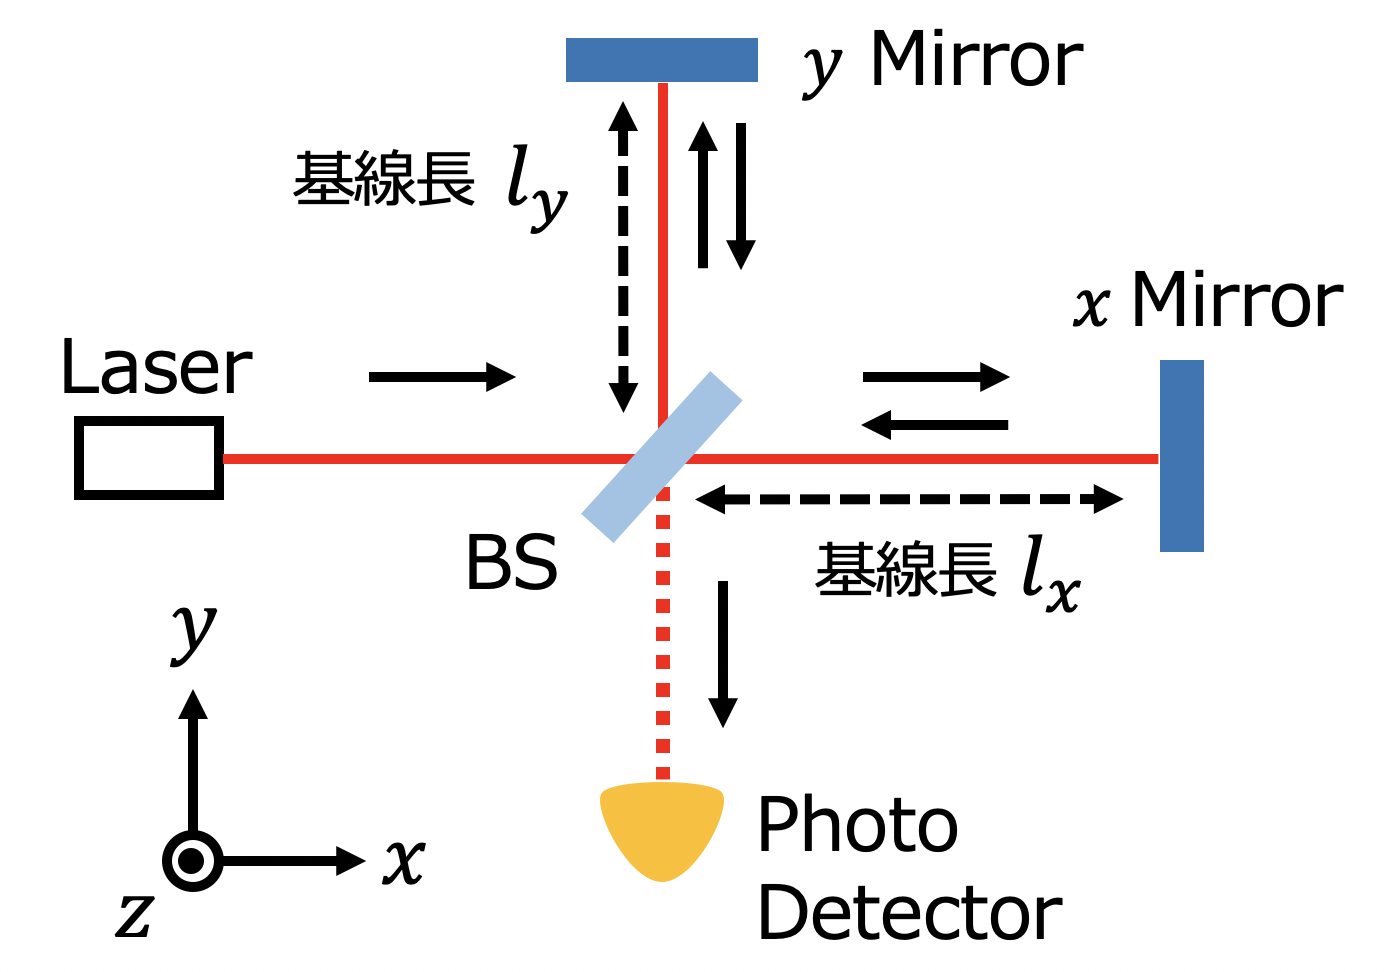
\includegraphics[width=110mm]{fig2_2.png}
\caption[Michelson干渉計]{Michelson干渉計(レーザー干渉計型重力波検出器の基本構成)の概念図}
\label{fig2.2}
\end{center}
\end{figure}
この干渉計に重力波が到来すると自由質点間(観測周波数帯域において自由質点となるよう, 鏡は振り子型の懸架装置に吊るされている)の固有距離(BSと$x,y$ Mirror間の距離)が変化し, この光路長変化によってBSに戻ってくる光に位相変調が加わる. これはキャリアである入射レーザー光に対して重力波の周波数に応じたSideband(側波帯)が生成されるということを意味している. 重力波信号を運ぶこのSidebandを信号Sidebandと呼ぶ. 信号Sidebandは二つの腕で逆位相となるので, BSでの干渉条件はレーザー光とは逆になる. つまり, 光が漏れていなかったSignal Portに信号Sidebandが抜けてくる. これを Photo Detector (PD) で検出することで, 重力波の到来が分かる. この様子を数式で示すと以下のようになる. \\
\quad レーザーから出た光を$E_0(t)=A{\rm e}^{i\Omega t}$とする(角周波数$\Omega$はレーザー光の波長$\lambda$を用いて$\Omega=2\pi c/\lambda$). BSで分かれた光は$x$ Mirrorおよび$y$ Mirrorで反射して再びBSに戻ってくる. ここで$y$ Mirrorで反射してPDに入る光が$x$ Mirrorによる反射光に対して$\delta\phi$だけ位相がずれるとするとPDで検出される光は
\begin{equation}
E_{\rm PD}(t)=E_x{\rm e}^{i\Omega t}-E_y{\rm e}^{i(\Omega t+\delta\phi)},
\end{equation}
と書ける($E_x,E_y$はそれぞれ$x,y$ Mirrorから返ってくる光の振幅). これよりPDで受け取る光の強度は
\begin{equation}
P=\left|E_{\rm PD}(t)\right|^2=\frac{P_{\rm max}+P_{\rm min}}{2}+\frac{P_{\rm max}-P_{\rm min}}{2}\cos(\delta\phi),
\end{equation}
となる. ただし, 
\begin{equation}
P_{\rm max}=\frac{(E_x+E_y)^2}{2},\,\,P_{\rm min}=\frac{(E_x-E_y)^2}{2},
\end{equation}
である. よって位相差$\delta\phi$によって強度が余弦関数的に変化することが分かる. また, $P_{\rm max}$と$P_{\rm min}$を用いて
\begin{equation}
C\equiv\frac{P_{\rm max}-P_{\rm min}}{P_{\rm max}+P_{\rm min}},
\end{equation}
が定義される. これは干渉計のコントラストと呼ばれ, 完全に干渉状態にあるとき$C=1$, 全く干渉していないとき$C=0$となる. つまり, 干渉縞の明瞭度を表す指標である. 
\subsubsection{重力波に対する応答}
\vskip3mm
さて, 重力波$h_{+}$がMichelson干渉計へ$z$方向に入射したときの応答を考える. このとき
\begin{equation}
{\rm d}s^2=-c{\rm d}t^2+(1+h_+){\rm d}x^2+(1-h_+){\rm d}y^2+{\rm d}z^2,
\end{equation}
と書ける. $x,y$ Mirrorは自由質点であるから座標は変化せず, 光は${\rm d}s^2=0$の世界線を進むので$x$軸上において
\begin{equation}
{\rm d}x=\pm\frac{c{\rm d}t}{\sqrt{1+h_{+}}}\sim\pm\left(1-\frac{1}{2}h_+\right)c{\rm d}t,
\end{equation}
である. これをBSと$x$ Mirrorの間を往復する経路(所要時間$\tau_x$)で積分すると
\begin{equation}
\frac{2l_x}{c}=\int_{t-\tau_x}^t\left(1-\frac{1}{2}h_+\right){\rm d}t^{\prime},
\end{equation}
となる. ここで重力波の振幅は極めて小さい($h\ll1$)なので積分範囲の$\tau_x$は$2l_x/c$とみなせて
\begin{equation}
\tau_x=\frac{2l_x}{c}+\frac{1}{2}\int_{t-2l_x/c}^th_+{\rm d}t^{\prime},
\end{equation}
が得られる. これより$x$軸上で1往復する際の位相変化を求めると
\begin{equation}
\phi_x=\Omega\tau_x=\frac{2l_x\Omega}{c}+\frac{\Omega}{2}\int_{t-2l_x/c}^th_+{\rm d}t^{\prime}.
\end{equation}
$y$軸上の場合も符号が異なること以外は同様に計算できるので, $l_x\sim l_y\sim l$の場合の位相差は
\begin{equation}
\delta\phi=\frac{2(l_x-l_y)\Omega}{c}+\Omega\int_{t-2l_x/c}^th_+{\rm d}t^{\prime}.
\end{equation}
この式のうち, 第2項が重力波による位相変化$\delta\phi_{\rm GW}$であり, これを読み取ることで重力波の検出が可能になる. ここで$h_+(t)$のFourier変換
\begin{equation}
h_+(t)=\int_{-\infty}^{\infty}h_+(\omega){\rm e}^{i\omega t}{\rm d}\omega,
\end{equation}
を用いると重力波による位相変化は
\begin{equation}
\delta\phi_{GW}=\int_{-\infty}^{\infty}H_{\rm MI}h_+(\omega){\rm e}^{i\omega t}{\rm d}\omega.
\end{equation}
ただし, 
\begin{equation}
H_{\rm MI}=\frac{2\Omega}{c}\sin\left(\frac{l\omega}{c}\right){\rm e}^{-\frac{i\omega l}{c}},
\label{eq2.58}
\end{equation}
である. これがMichelson干渉計の重力波に対する周波数応答になる. この式より$|H_{\rm MI}|$が最大になるのは
\begin{equation}
\frac{l\omega}{c}=\frac{\pi}{2},
\end{equation}
のときであることが分かるが, これは重力波の位相が1往復でちょうど反転する場合にMichelson干渉計の感度が最も良くなることを表している. さらに, 100 Hzの重力波を観測する場合はおよそ750 kmの腕の長さを持つ干渉計が必要であることも分かる. しかし, そのような長さの干渉計を地上に建設することは不可能であるため, 光を何度も往復させて実行的な光路長を長くするFabry-Perot型の干渉計が用いられる. 
\subsection{Fabry-Perot Michelson干渉計}
\subsubsection{Fabry-Perot共振器}
\label{sec2.2.2.1}
\begin{figure}[H]
\begin{center}
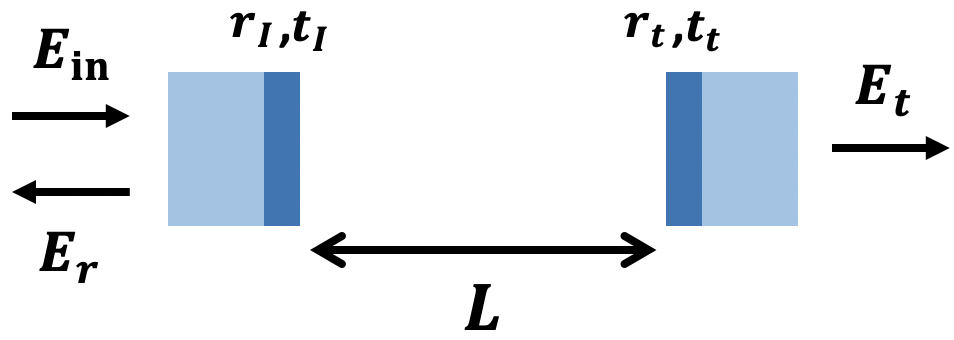
\includegraphics[width=120mm]{fig2_3.png}
\caption[Fabry-Perot Michelson共振器]{Fabry-Perot 共振器}
\label{fig2.3}
\end{center}
\end{figure}
Fabry-Perot Michelson干渉計の原理や重力波に対する応答を記す前に, Fabry-Perot共振器について概要を記す. \\
\quad 図\ref{fig2.3}のような長さ$L$のFabry-Perot共振器を考え, ITMの振幅反射率および透過率を$r_I$, $t_I$とし, ETMに対しても同様に$r_E$, $t_E$とする. このとき, 共振器の反射光電場は
\begin{equation}
E_r=-r_IE_{\rm in}+\sum\limits_{n=1}^{\infty}t_I^2r_I^{n-1}r_E^{n}{\rm e}^{i\times2nkL}E_{\rm in}=\left(-r_I+\frac{t_I^2r_E{\rm e}^{2ikL}}{1-r_Ir_E{\rm e}^{2ikL}}\right)E_{\rm in},
\end{equation}
\begin{equation}
E_t=\sum\limits_{n=1}^{\infty}t_It_Er_I^{n-1}r_E^{n-1}{\rm e}^{i\times(2n-1)kL}E_{\rm in}=\frac{t_It_E{\rm e}^{2ikL}}{1-r_Ir_E{\rm e}^{2ikL}}E_{\rm in},
\end{equation}
となる. よって共振器の振幅反射率・透過率 ($r_{cav}$, $t_{cav}$) と強度反射率・透過率 ($R_{\rm cav}$, $T_{\rm cav}$) は
\begin{align}
r_{\rm cav}&=\frac{E_r}{E_{\rm in}}=-r_I+\frac{t_I^2r_E{\rm e}^{2ikL}}{1-r_Ir_E{\rm e}^{2ikL}}\label{eq2.62}\\
t_{\rm cav}&=\frac{E_t}{E_{\rm in}}=\frac{t_It_E{\rm e}^{2ikL}}{1-r_Ir_E{\rm e}^{2ikL}}\label{eq2.63}\\
R_{\rm cav}&=\left|r_{\rm cav}\right|^2=\frac{\left[r_I-(r_I^2+t_I^2)r_E\right]^2+4r_Ir_E(r_I^2+t_I^2)\sin^2kL}{(1-r_Ir_E)^2+4r_Ir_E\sin^2kL}\label{eq2.64}\\
T_{\rm cav}&=\left|t_{\rm cav}\right|^2=\frac{(t_It_E)^2}{(1-r_Ir_E)^2+4r_Ir_E\sin^2kL},
\label{eq2.65}
\end{align}
であり, さらに入射光強度に対する共振器内の光強度は式(\ref{eq2.65})の分子において$t_E^2$で割って, 
\begin{equation}
T_{\rm cav内}=\frac{t_I^2}{(1-r_Ir_E)^2+4r_Ir_E\sin^2kL},
\label{eq2.66}
\end{equation}
と表される. なお, 鏡の反射・透過による光学的な損失がない場合は$r_I^2+t_I^2=1$であり, $R_{\rm cav}+T_{\rm cav}=1$となる. \\
\quad 式(\ref{eq2.65})において$kL=n\pi\,\,(n\in{\bm{N}})$とすると強度透過率は最大値$T_{\rm cav}^{\rm max}=\frac{(t_It_E)^2}{(1-r_Ir_E)^2}$をとり, この状態を共振状態と呼ぶ. 一方, $kL=(n+\frac{\pi}{2})$のとき, 強度透過率は最小値$T_{\rm cav}^{\rm min}=\frac{(t_It_E)^2}{(1+r_Ir_E)^2}$となり, 反共振状態と呼ばれる. \\
\quad ここで, 強度透過率をレーザー周波数の関数とみなすと, 隣り合う共振状態の周波数差は式(\ref{eq2.65})より
\begin{equation}
\nu_{\rm FSR}=\frac{c}{2L},
\end{equation}
と表され, フリースペクトラルレンジ (Free Spectral Range : FSR) と呼ばれる. また, Fabry-Perot共振器を構成する鏡の反射率が1に近い時は$T_{\rm cav(\nu)}$は$\nu_{\rm FSR}$間隔で鋭いピークを持つ(図\ref{fig2.4}). このピークの半値全幅を$\nu_{\rm FWHM}(r_I,r_E)$とすると, 
\begin{equation}
T_{\rm cav}(\nu_{\rm FWHM})=\frac{1}{2}T_{\rm cav}^{\rm max},
\end{equation}
であり, 
\begin{equation}
\nu_{\rm FWHM}(r_I,r_E)=\frac{c(1-r_Ir_E)}{2\pi L\sqrt{r_Ir_E}},
\end{equation}
と書ける. ここで$\nu_{\rm FSR}$と$\nu_{\rm FWHM}$の比をとると, 
\begin{equation}
\mathcal{F}(r_I,r_E)=\frac{\nu_{\rm FSR}}{\rm FWHM}=\frac{\pi\sqrt{r_Ir_E}}{1-r_Ir_E},
\label{eq2.70}
\end{equation}
となる. この$\mathcal{F}$はフィネスと呼ばれ, Fabry-Perot共振器の共振の鋭さを表している. 
\begin{figure}[H]
\begin{center}
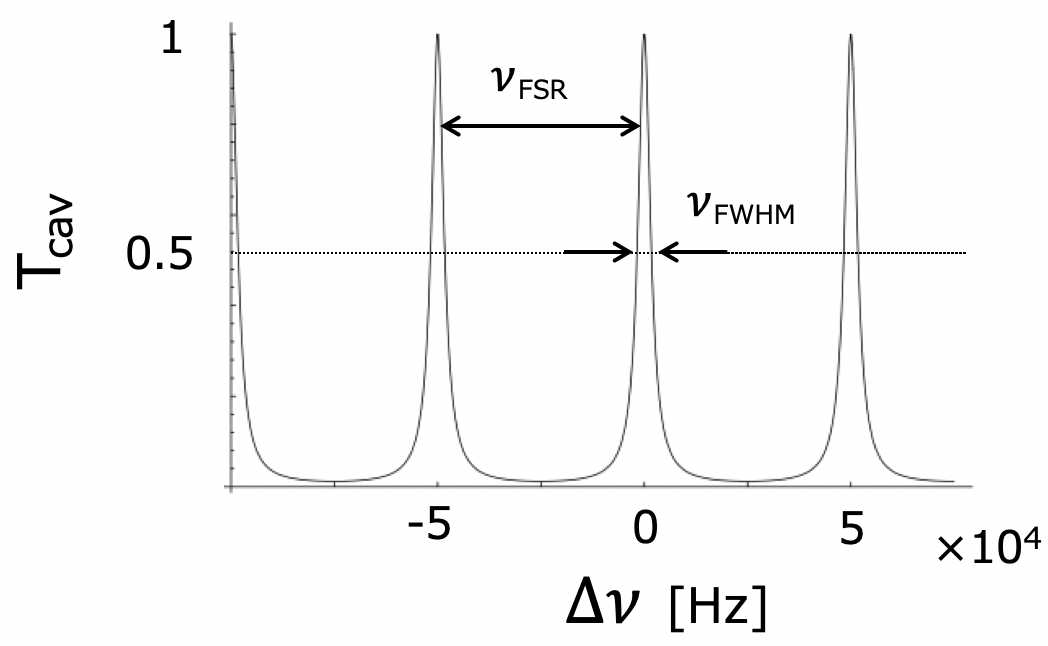
\includegraphics[width=120mm]{fig2_4.png}
\caption[Fabry-Perot共振器の強度透過率]{Fabry-Perot共振器の強度透過率. 横軸はある共振周波数からのずれである. また, 縦軸は適当な値に規格化してある. }
\label{fig2.4}
\end{center}
\end{figure}
\subsubsection{原理}
\vskip3mm
Fabry-Perot Michelson干渉計 (Fabry-Prrot Michelson Interferometer : FPMI) は図\ref{fig2.5}に示したように, Michelson干渉計のBSと各鏡の間にもう1つずつ鏡を入れた構成になっている. 各腕の2個の鏡で構成された共振器がFabry-Perot共振器であり, 向かい合う鏡間の距離を光の波長の半整数倍に調整して光を共振させている. \\
\quad FPMIではBSから入射した光は, 一部の光が透過するような薄膜コーティングが施された Input Test Mass (ITM)を透過し, ほぼすべての光が反射するような薄膜コーティングがなされた End Test Mass (ETM) で反射し, 再びITMに戻る. また, 鏡の共振器側は反射コーティングがなされているため, ETMからITMへ戻ってきた光は再度ETMへ反射される. このコーティングの反射率を調整して共振器内の光が少しずつBS側に滲み出ていくようにすることで, 光はある平均折り返し回数$n$で共振器の外へと出ていくとみなせるようになる. 
\begin{figure}[H]
\begin{center}
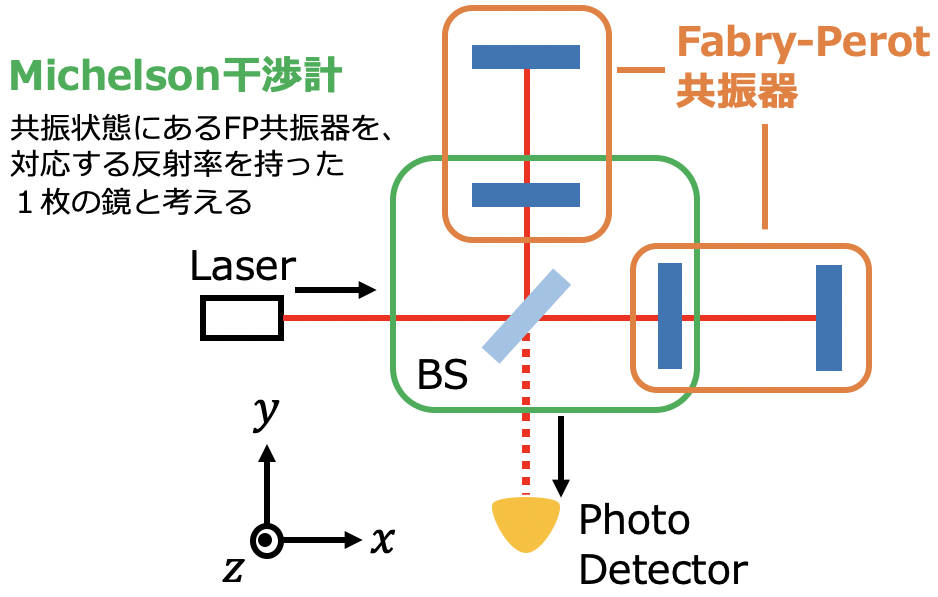
\includegraphics[width=120mm]{fig2_5.png}
\caption[Fabry-Perot Michelson干渉計]{Fabry-Perot Michelson干渉計の概念図}
\label{fig2.5}
\end{center}
\end{figure}
\subsubsection{重力波に対する応答}
\vskip3mm
先ほどと同様に, 重力波$h_{+}$がFPMIへ$z$方向に入射したときの応答を考える. 光が$\tau_n$の時間をかけて共振器を$n$回往復したとすると
\begin{equation}
\tau_n=\frac{2L}{c}n+\frac{1}{2}\int_{-\infty}^{\infty}h_+(\omega)\frac{1-{\rm e}^{-2inL\omega/c}}{i\omega}{\rm e}^{i\omega t}{\rm d}\omega,
\end{equation}
となる. ここで, ITMの反射率および透過率を$r_I,t_I$, ETMの反射率を$r_E$とし, 光が共振器長$L$だけ進んだときの位相変化を$\Delta$とするとFabry-Perot共振器内で反射される光の振幅は
\begin{equation}
E_r=E_0\left(r_I-t_I^2r_E\sum_{n=0}^{\infty}r_I^{n}r_E^{n}\right){\rm e}^{-2in\Delta},
\end{equation}
と書ける. 共振しているときは$\Delta=n\pi$なので$h$の1次まで計算すると
\begin{equation}
E_r\sim E_0\frac{r_I-r_E(t_I^2+r_I^2)}{1-r_Ir_E}\left(1-i\int_{-\infty}^{\infty}H_{\rm FP}(\omega)h_+(\omega){\rm e}^{i\omega t}{\rm d}\omega\right),
\end{equation}
となる. ただし, 
\begin{equation}
H_{\rm FP}=\frac{2\alpha\Omega}{\omega}\frac{\sin(\omega L/c)}{1-r_Ir_E{\rm e}^{-2i\omega L/c}}{\rm e}^{-i\omega L/c},
\end{equation}
\begin{equation}
\alpha=\frac{t_I^2r_E}{r_I-(r_I^2+t_I^2)r_E},
\end{equation}
である. この$H_{\rm FP}$がFPMIの周波数応答を示し, 
\begin{equation}
|H_{\rm FP}|=\frac{2\alpha\Omega}{\omega(1-r_Ir_E)}\frac{|\sin(\omega L/c)|}{\sqrt{1+F\sin^2(\omega L/c)}},
\end{equation}
となる. ここで$F$はフィネスを用いて
\begin{equation}
F=\frac{4r_Ir_E}{(1-r_Ir_E)^2}=\frac{2\mathcal{F}}{\pi},
\end{equation}
と表される値である. \\
\quad また, 光が共振器内を動く間の重力波の時間変化が十分小さい, すなわち$\omega L/c\ll 1$のときは
\begin{equation}
\begin{split}
|H_{\rm FP}|&\simeq\frac{2\alpha\Omega}{\omega(1-r_Ir_E)}\frac{\omega L/c}{\sqrt{1+F(\omega L/c)^2}}\\
&=\frac{2\alpha\Omega L}{c(1-r_Ir_E)}\frac{1}{\sqrt{1+\left(\frac{\sqrt{F}L}{c}\omega\right)^2}}\\
&=\frac{2\alpha\Omega L}{c(1-r_Ir_E)}\frac{1}{\sqrt{1+\left(\frac{\omega}{\omega_c}\right)^2}}
\end{split},
\label{eq2.78}
\end{equation}
となり, キャビティポール$2\pi\omega_c$の1次のローパス特性を保つことが分かる. ここで, 
\begin{equation}
\omega_c=\frac{c}{\sqrt{F}L}=\frac{c(1-r_Ir_E)}{2L\sqrt{r_Ir_E}},
\end{equation}
であり, 
\begin{equation}
\nu_c=\frac{\omega_c}{2\pi}=\frac{c(1-r_Ir_E)}{4\pi L\sqrt{r_Ir_E}}=\frac{1}{2}\nu_{\rm FWHM},
\end{equation}
は cut-off 周波数である. また, キャビティポールの逆数
\begin{equation}
\tau=\frac{1}{\omega_c}=\frac{2L\sqrt{r_Ir_E}}{c(1-r_Ir_E)},
\end{equation}
は光が共振器内に滞在する平均時間 (strage time) を表す. この平均滞在時間は式(\ref{eq2.70})を用いて
\begin{equation}
\tau=\frac{2L}{\pi c}\mathcal{F},
\label{eq2.82}
\end{equation}
と表せる. 一方, Fabry-Perot共振器における折り返し数を$N_{\rm FP}$とすると
\begin{equation}
\tau=N_{\rm FP}\frac{2L}{c},
\end{equation}
なので, 式(\ref{eq2.82})と合わせて
\begin{equation}
N_{\rm FP}=\frac{\mathcal{F}}{\pi},
\end{equation}
となり, 折り返し数をフィネスで表すことができる. \\
\quad 最後にMichelson干渉計の場合と比較する. 重力波に対する周波数応答の比を取ると, 式(\ref{eq2.58})と式(\ref{eq2.78})より, 
\begin{equation}
\frac{\left|H_{\rm FP}\right|}{\left|H_{\rm MI}\right|}=\frac{2\alpha}{1-r_Ir_E}\frac{1}{\sqrt{1+\left(\frac{\omega}{\omega_c}\right)^2}},
\end{equation}
となる. この式において$r_E\rightarrow 1,\omega\ll\omega_c$とすると
\begin{equation}
\frac{\left|H_{\rm FP}\right|}{\left|H_{\rm MI}\right|}\rightarrow\frac{4}{T_I},
\end{equation}
であり, この極限で FPMIは実効的にアーム長が$4/T_I$のMichelson干渉計とみなすことができる. また, 両者の周波数応答を図\ref{fig2.6}に示した. 低周波ではFPMIの腕共振器の影響により, Michelson干渉計よりも応答が増幅されるが, キャビティポール(cut-off 周波数)より高周波では信号が減衰されてしまう. 
\begin{figure}[H]
\begin{center}
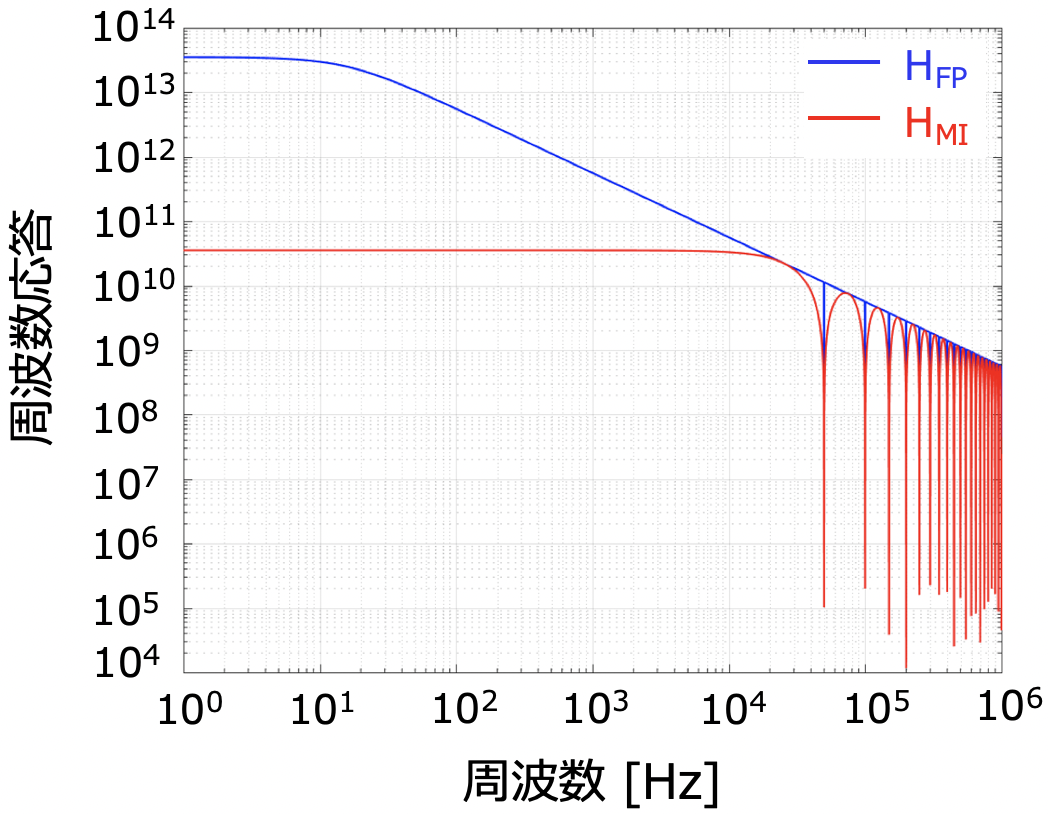
\includegraphics[width=130mm]{fig2_6.png}
\caption[Michelson干渉計とFPMIの周波数応答]{Michelson干渉計 (3 km) とFPMI (腕共振器の長さ3 km) の周波数応答. 低周波において, FPMIでは腕共振器の影響で, Michelson干渉計よりも応答が増幅される. しかし, キャビティポール(cut-off 周波数)より高周波では信号が減衰されてしまう.  }
\label{fig2.6}
\end{center}
\end{figure}
\subsection{DRFPMI}
FPMIにパワーリサイクリングとRSEを導入した干渉計を Dual-Recycled Fabry-Perot Michelson Interferimeter (DRFPMI) と呼び, 現在はこの形がレーザー干渉計型重力波検出器の主流なものとなっている. なお図\ref{fig2.7}に示したように, DRFPMIには全部で5つの長さ自由度がある. \\
\quad まず, DARMと呼ばれるのはFabry-Perot共振器の差動変動であり, 重力波信号はこの自由度の変動として現れる. 一方CARMはFabry-Perot共振器長の同相成分である. CARMの信号は共振器長変動の同相成分であり, レーザーの周波数揺らぎを反映するようになっているので, この自由度を用いてレーザー周波数の安定化を行う. また, PRCLおよびSRCLはPower Recycling Cavity (PRC), Signal Recycling Cavity (SRC) の長さであり, それぞれ2枚のITMとPower Recycling Mirror (PRM), Signal Recycling Mirror (SRM) の距離の平均で表される. 最後に, MICHとはMichelson干渉計部分の自由度である. 以下ではパワーリサイクリングとRSEについて簡単に記す. 
\begin{figure}[H]
\begin{center}
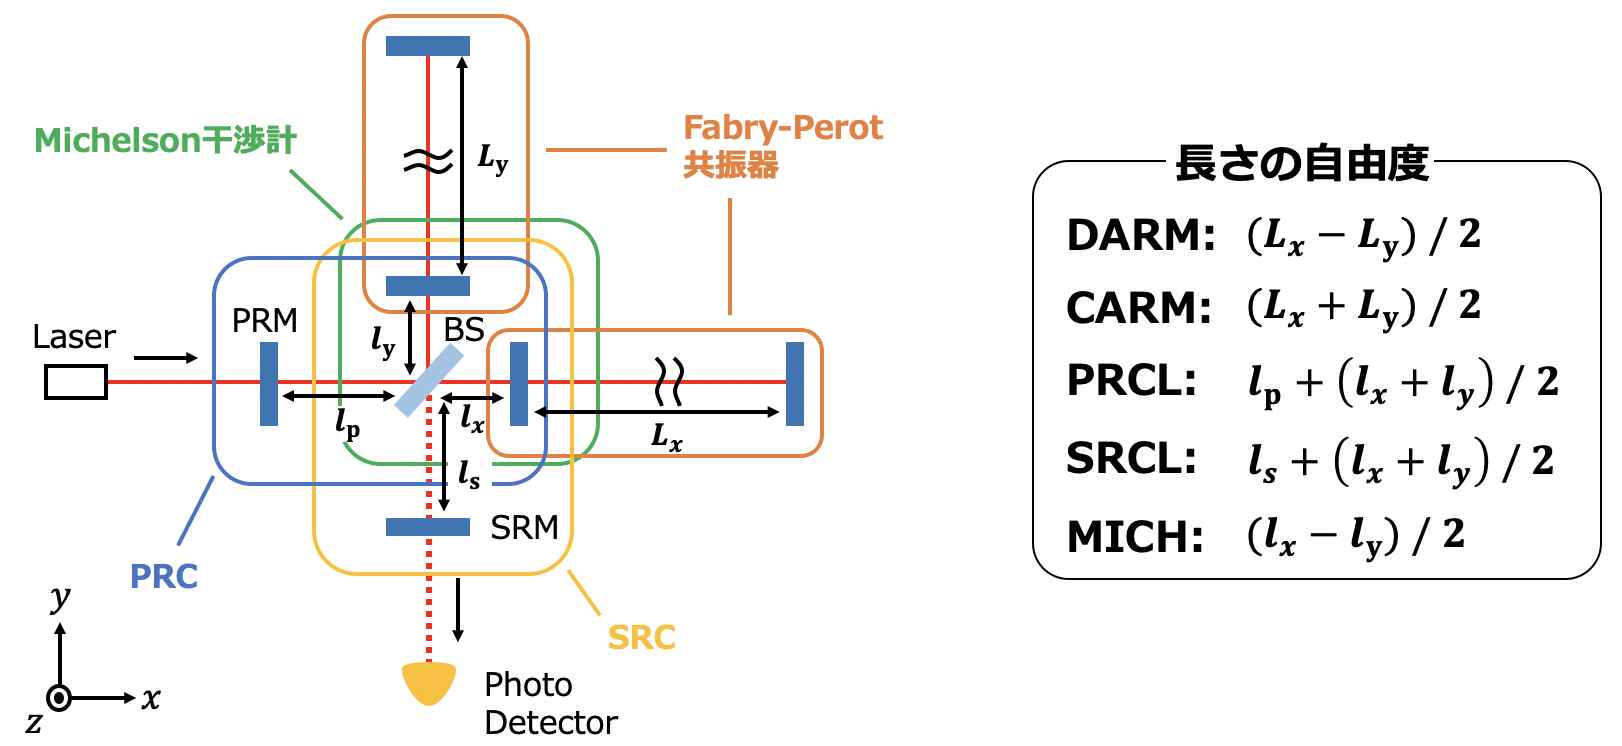
\includegraphics[width=170mm]{fig2_7.png}
\caption[DRFPMI干渉計]{DRFPMI干渉計の概念図および長さの自由度}
\label{fig2.7}
\end{center}
\end{figure}
\subsubsection{パワーリサイクリング}
\vskip3mm
重力波検出器では, 散射雑音の最小化のため, 干渉計のSignal Portから光が漏れないような制御をしている. そのため, レーザーパワーのほとんどが入射側へと戻っていく. 一方, 重力波信号を大きくするためには重力波と相互作用する腕共振器内のレーザーパワーを上げる必要がある. そこで, 戻っていくレーザーをFPMIに打ち返す鏡を入射側に置き, 実効的なレーザーパワーを増大させている. これにより, 散射雑音レベルを改善することができる\cite{power}. \\
\quad この手法をパワーリサイクリングと呼び, 打ち返しを行う鏡を Power Recycling Mirror (PRM) と呼ぶ(図\ref{fig2.7}). このとき, 入射側から見たFPMIは全体として1つの鏡とみなすことができる(レーザーをPRM側に反射している). ここで, 光共振器において, 二つの鏡の反射率が等しい場合, 入射したレーザーパワーは内部で熱に変わるか, あるいは透過する. しかし, 重力波検出器ではETMの反射率が極めて高いので, ほとんどの光は熱に変換されるまでの間, 干渉計内にとどまる. よって, FPMIを1つの鏡とみなしたときの反射率とPRMの反射率を一致させることで, 入射レーザーパワーを最大効率で利用できるのである. \\
\quad また, 2つのITMとPRMで構成される共振器は Power Recycling Cavity (PRC) と呼ばれる. このPRCはPRMと腕共振器の複合鏡からなる共振器とみなせる. そこで, 式(\ref{eq2.66})において$r_I\rightarrow r_P$, $t_I\rightarrow t_P$, $r_E\rightarrow r_{\rm Acav}$, $L\rightarrow l_p$と置き換えると, 入射光電場$E_{\rm in}$に対する, BSでの光電場$E_{\rm BS}$の強度増幅率$G_P$が得られる. なお, $r_p$, $t_p$はPRMの振幅反射率および振幅透過率, $r_{\rm Acav}$は腕共振器の振幅反射率である. パワーリサイクリングでは, 光電場がPRC長$l_{P}$に対して共振状態となるようにするので
\begin{equation}
G_P=\frac{t_P^2}{\left(1-r_Pr_{\rm Acav}\right)^2},
\end{equation}
となる. ここで, 共振器の振幅反射率を表した式(\ref{eq2.62})において, 共振状態を考えるとPRCに対して
\begin{equation}
r_{\rm PRC}=\frac{-r_P+\left(r_P^2+t_P^2\right)r_{\rm Acav}}{1-r_Pr_{\rm Acav}},
\end{equation}
である. 光学損失がないとすると, $r_P=r_{\rm Acav}$のときに$r_{\rm PRC}=0$となるのでこれが最適条件であり, このとき$G_P$は
\begin{equation}
G_P=\frac{1}{t_P^2}=\frac{1}{T_P},
\end{equation}
となり, PRMの強度透過率に反比例する. なお, $G_P$はパワーリサイクルゲインと呼ばれ, KAGRAではこの値は10となっている. 
\subsubsection{Resonant Sideband Extraction}
\vskip3mm
Fabry-Perot共振器のフィネスを上げることで光子の折り返し数が増え, 重力波信号が増幅されるが, 1つの光子が共振器内に留まっている間に重力波の符号が反転してしまう. これにより光子に蓄積された位相変化がキャンセルされ, 高周波で重力波信号に対する感度が落ちてしまう. そこで Resonant Sideband Extraction (RSE) と呼ばれる手法を用いる\cite{RSE}. \\
\quad RSEでは Signal Recycling Mirror (SRM) がSignal Port側に置かれる(図\ref{fig2.7}). この鏡とFabry-Perot共振器のITM2枚で Signal Recycling Cavity (SRC) を構成しており, 重力波が入射したときに生成される信号SidebandがSRCに共振するようにSRCの長さを制御している. このとき, 信号SidebandにとってのSRCの反射率(Fabry-Perot共振器内から見たITMの反射率)はITM単体よりも低くなる. よって信号Sidebandに対するFabry-Perot共振器の実効的なフィネスが下がる, すなわち信号SidebandだけFabry-Perot共振器内の滞在時間が減り, 高周波での信号減衰の程度が小さくなる. なお, レーザー光にとってはFabry-Perot共振器のフィネスは高いままなので, 重力波信号の増幅率は変わらない. \\
\quad また, SRCはキャリアに対して共振もしくは反共振に制御するかの違いで, それぞれBroad Resonant Sideband Extraction (BRSE), Broadband Signal Recycling (BSR) と呼ばれる(図\ref{fig2.8}). \\
\quad BRSEではSRMとITMの複合鏡の振幅反射率が小さくなり, 腕共振器でのキャリアの平均往復回数が小さくなるため, 低周波において信号増幅率が低下する. 一方, 高周波では信号が相殺する前に腕共振器から抜き出すことで, 信号を増幅している(signal extraction). BSRではその全く逆で, 低周波では信号増幅率が高く (signal recycling), 高周波では信号相殺の影響が大きくなる. これをまとめると, BRSEとBSRの周波数応答は図\ref{fig2.9}のようになる. 
\begin{figure}[H]
\begin{center}
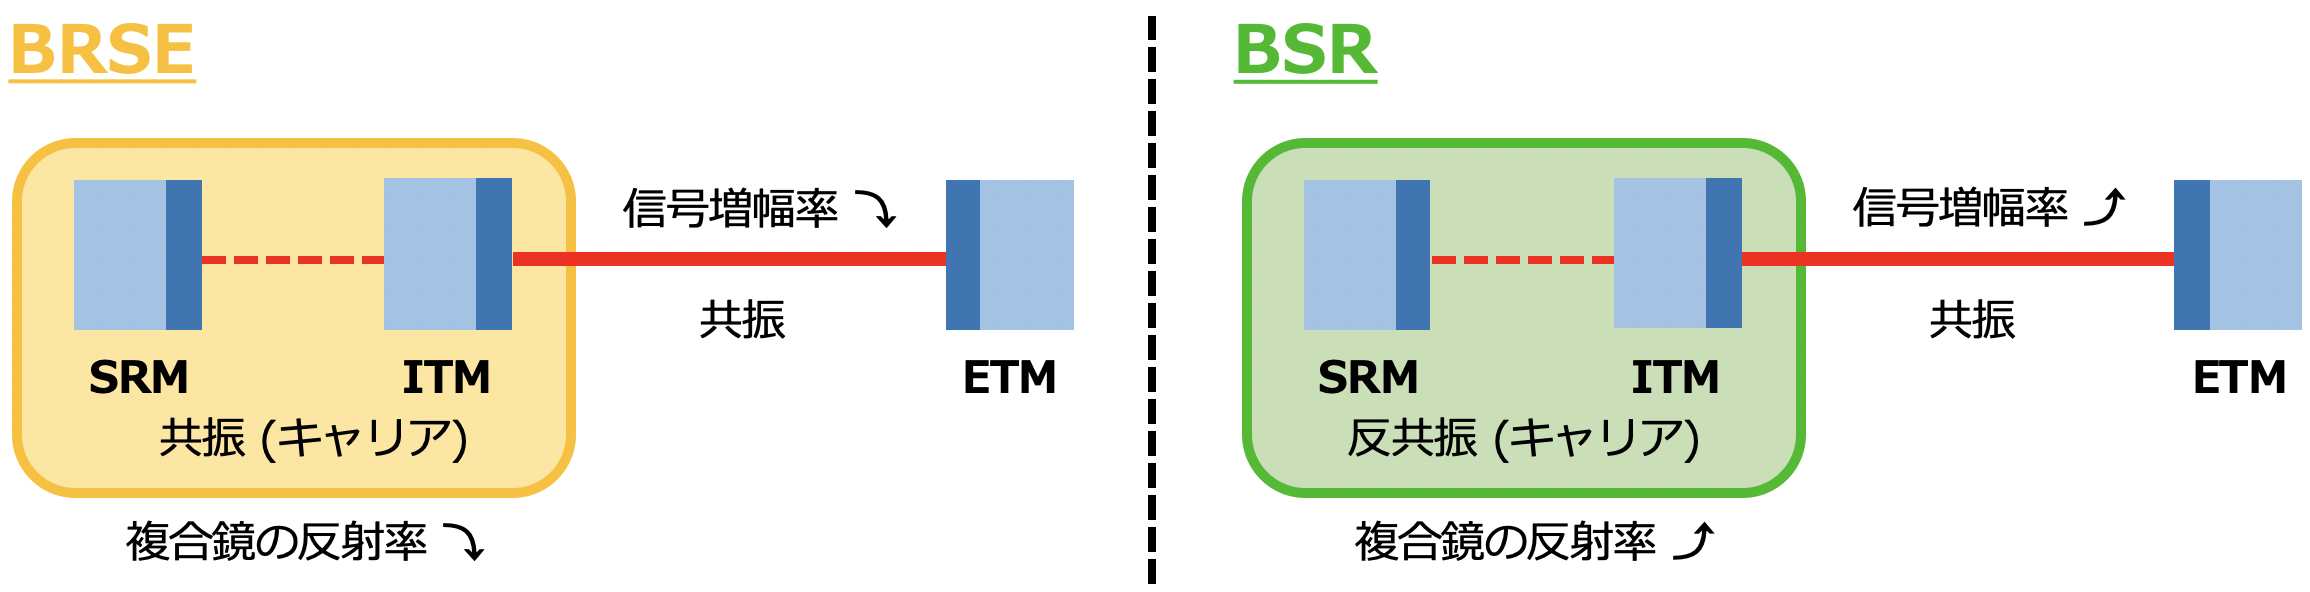
\includegraphics[width=170mm]{fig2_8.png}
\caption[SRCのモード]{SRCのモード. BRSEではSRMとITMの複合鏡の振幅反射率が小さくなり, 腕共振器でのキャリアの平均往復回数が小さくなるため, 低周波において信号増幅率が低下する. 一方で, 高周波では信号が増幅される. BSRではその逆となる. }
\label{fig2.8}
\end{center}
\end{figure}
\begin{figure}[H]
\begin{center}
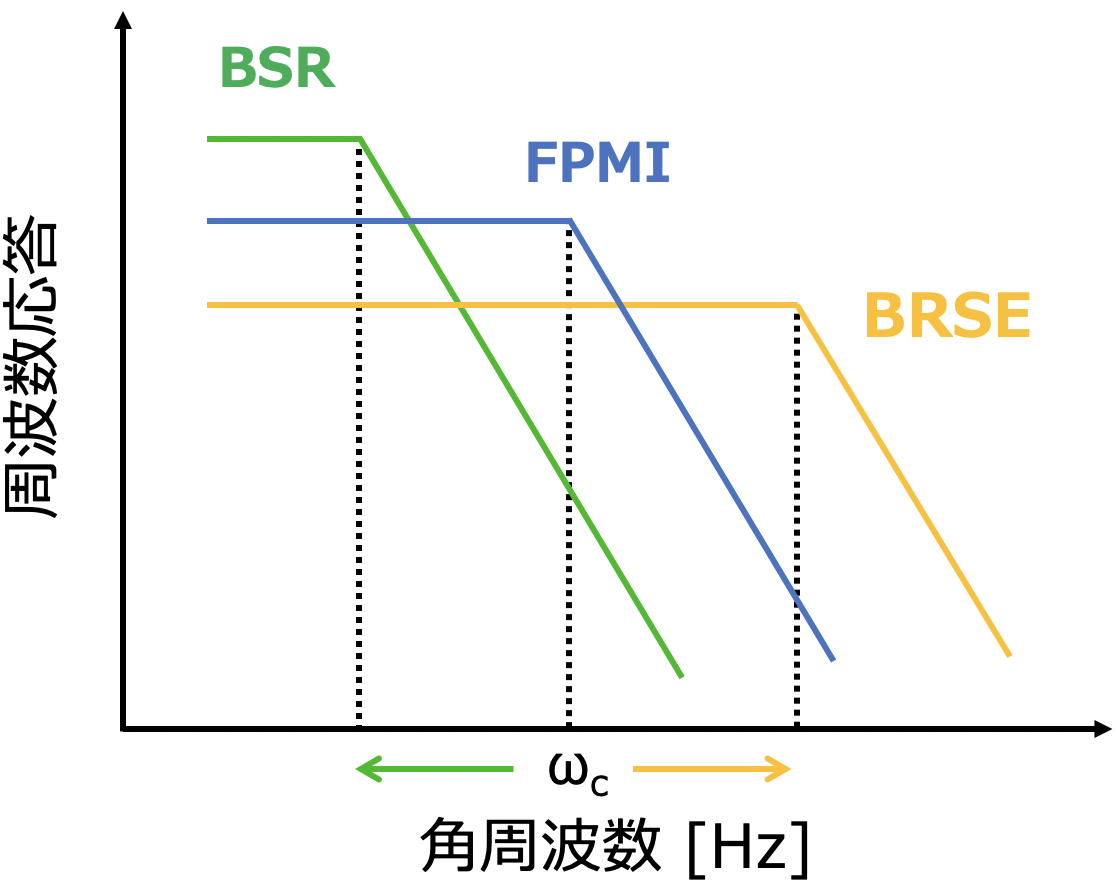
\includegraphics[width=110mm]{fig2_9.png}
\caption[光の散射雑音スペクトルの概念図]{重力波に対する周波数応答の比較. BRSEではFPMIに比べ, 低周波において信号増幅率が低下する一方で, 高周波において信号相殺の影響が小さくなる. BSRではその逆となる. }
\label{fig2.9}
\end{center}
\end{figure}
\subsection{レーザー干渉計型重力波検出器の雑音源}
重力波による長さ変動は小さく, 重力波検出器は種々の雑音に感度を制限される(図\ref{fig2.10}). ここでは干渉計の感度を決める基本的な雑音源をまとめる. 
\begin{figure}[H]
\begin{center}
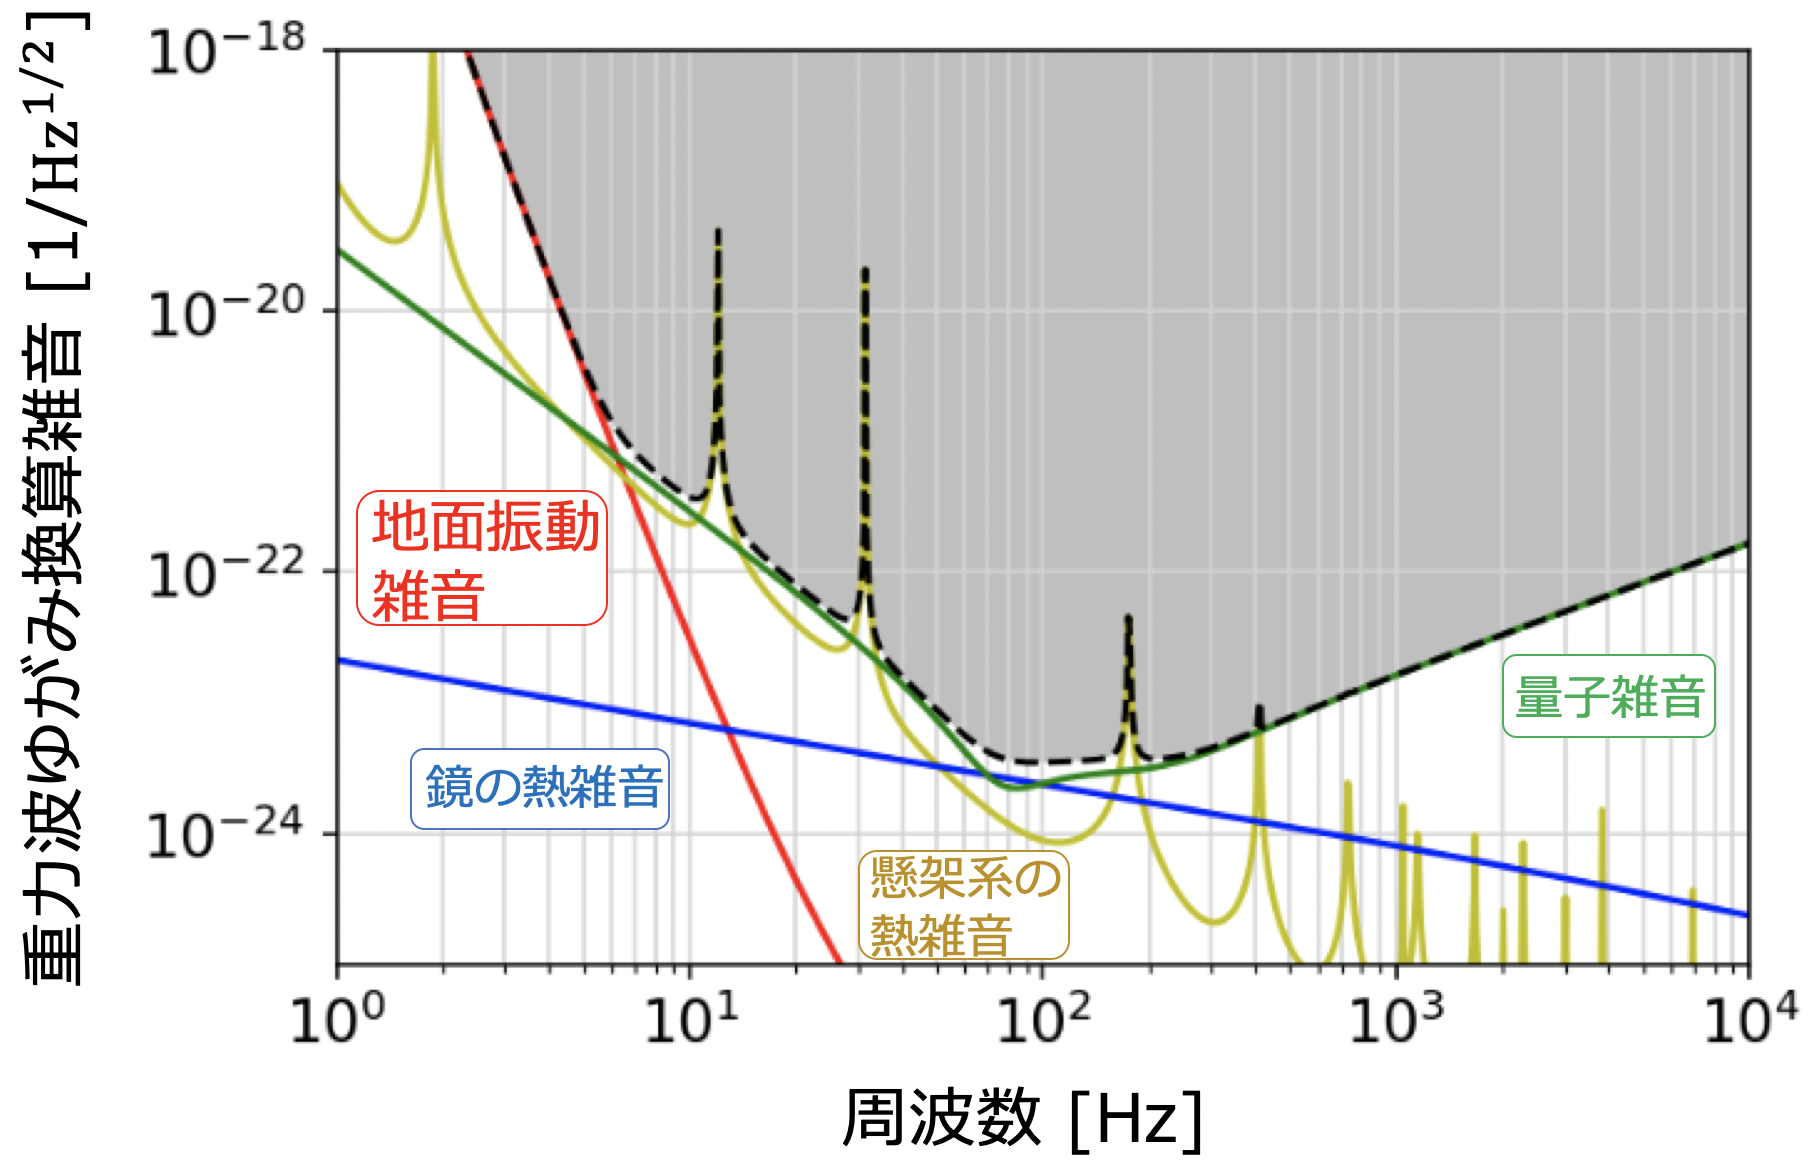
\includegraphics[width=140mm]{fig2_10.png}
\caption[KAGRAの感度曲線]{KAGRAの感度曲線. 10 Hz以下の低周波では主に地面振動や懸架系の熱雑音によって感度が制限される. また, 量子雑音は広い帯域で感度を制限している. }
\label{fig2.10}
\end{center}
\end{figure}
\subsubsection{量子雑音}
\vskip3mm
干渉計による重力波検出には, レーザー出力に起因する量子雑音がある. 量子非破壊測定を行わない場合, 量子雑音は光の位相の量子的揺らぎに起因する散射雑音と振幅の揺らぎに起因する輻射圧雑音に分けられる. \\
\quad 散射雑音は, レーザービーム中の光子数の量子的な揺らぎによって生じるノイズである. 検出器の出力に現れる重力波の信号は干渉計への入射パワー$P_0$に比例し(\ref{sec2.2.2.1}節), PDでの光子数の量子揺らぎは$\sqrt{P_0}$に比例する. よって, 重力は信号へと換算した散射雑音は$1/\sqrt{P_0}$に比例する. これより, 干渉計に入射するレーザーのパワーを上げることで散射雑音を低減することができる. なお, 散射雑音は約100 Hz以上の高周波帯で感度を制限している\cite{LIGO}. \\
\quad 一方, 輻射圧雑音は鏡の表面に作用する輻射圧の揺らぎによって発生するノイズである. このとき, 鏡に加わる力の量子揺らぎは$\sqrt{P_0}$に比例するため, 輻射圧雑音は$\sqrt{P_0}/m$に比例する. よって, 鏡の質量を大きくするか, 入射レーザーパワーを下げることで輻射圧雑音を改善することができる. なお, 輻射圧雑音は数10 Hz帯で感度を制限している\cite{LIGO}. \\
\quad これより, 散射雑音と輻射圧雑音は量子揺らぎはレーザーパワーに対して反対の依存性を持つため, 干渉計の感度への寄与はトレードオフの関係となる. また, この関係から導かれる量子雑音の下限は標準量子限界 (SQL) と呼ばれている. このSQLを超えるためには, 周波数依存性スクイージングやホモダイン検波によって量子雑音(特に輻射圧雑音)を低減するなどの方法がある\cite{24}. 
\subsubsection{熱雑音}
\vskip3mm
有限温度での原子の熱振動は鏡の表面軸位置や弾性形状の変動を引き起こし, 干渉計の光路長変動に関わる. この雑音を一般に熱雑音と呼ぶ. \\
\quad 重力波望遠鏡における熱雑音にもさまざまなものがある. 例えば熱浴とのやり取りによって懸架ファイバーの物理的振動が励起される\cite{25}. これについて, 有限温度$T$の熱浴に接した物体では, $k_BT$のエネルギーがその物体の各振動モードに分配され, 機械的な振動を行う. このとき熱振動のパワースペクトルは揺動散逸定理\cite{26}より, 
\begin{equation}
S_x(f)=-\frac{4k_BT}{2\pi f}{\rm Im}[H(2\pi f)],
\end{equation}
と表される. ただし, $k_B$はBoltzmann定数, $T$は刑が接する熱浴の温度, $H$は系が受ける外力から変位への伝達関数, $f$は周波数である. これより, 例えば
\begin{equation}
H(2\pi f)=\frac{1}{m(2\pi)^2\left[f_0^2(1+i\phi(f))-f^2\right]},
\end{equation}
という伝達関数で表された振動子の熱振動のパワースペクトルは
\begin{equation}
S_x(f)=-\frac{4k_BT}{m(2\pi)^3f}\frac{f_0^2\phi(f)}{(f^2-f_0^2)^2+f_0^4\phi^2(f)},
\end{equation}
となる. ここで, $\phi(f)$は散逸と呼ばれ, 振動子のエネルギー損失を特徴付ける量である. また, 散逸にはviscous damping(系の速度に比例した抵抗力が働くモデル)とstructure damping(材質に固有の構造減衰モデル)の2種類のモデルがあり, それぞれの場合で
\begin{equation}
\phi_v(\omega)=\frac{\omega}{\omega_0Q},
\end{equation}
\begin{equation}
\phi_s(\omega)=\frac{1}{Q},
\end{equation}
と表される. ただし, Qは共振の鋭さを表すパラメータであり, この値が大きいほど振動のエネルギーはピークに押し込められる. \\
\quad また, 懸架した鏡に入射するレーザーによる熱は, 懸架ファイバーを通して懸架系の上段へ伝えられる. そして, その熱はいくつかのステージを経由して冷却器へ流れる. このとき懸架ファイバーには下段から上段にかけて温度勾配が形成されるが, その温度勾配が緩和される際に変形を生じる. これは熱弾性雑音 (thermoelastic noise) と呼ばれている\cite{27}. \\
\quad 熱雑音を低減するためには鏡や懸架系の部品に機械的損失の小さな材料を選択する必要がある. 重力波望遠鏡の中には室温での機械的損失が小さい, すなわち機械的Q値が高い(約$10^7$)という理由で, 鏡の基材や懸架系ファイバーの材料として石英を採用しているものがある\cite{LIGO}. さらに, 温度を下げるという方法も考えられ, KAGRAではこの方法を採用している. 極低温環境下において, 溶融石英は優れた性能を示さないため, 極低温でも高い機械的Q値を示すサファイアが鏡基材として採用されている\cite{KAGRA}. \\
\quad なお, 鏡の基材やコーティング層の機械的損失や熱伝導率, 熱膨張率などの物性的性質に起因するものを鏡の熱雑音, 懸架系のワイヤ由来のものを懸架系の熱雑音と呼んでいる (図\ref{fig2.10}). \\
\subsubsection{地面振動雑音}
\vskip3mm
地球上に建設された重力波検出器にとって, 地面振動による雑音は避けられないものである. 地面は地震がない場合でもあらゆる周波数で微小振動しており, その連続的かつ不規則な地盤の運動は常に鏡を揺らす. その結果, 光共振器の長さが変動する. 
\begin{figure}[H]
\begin{center}
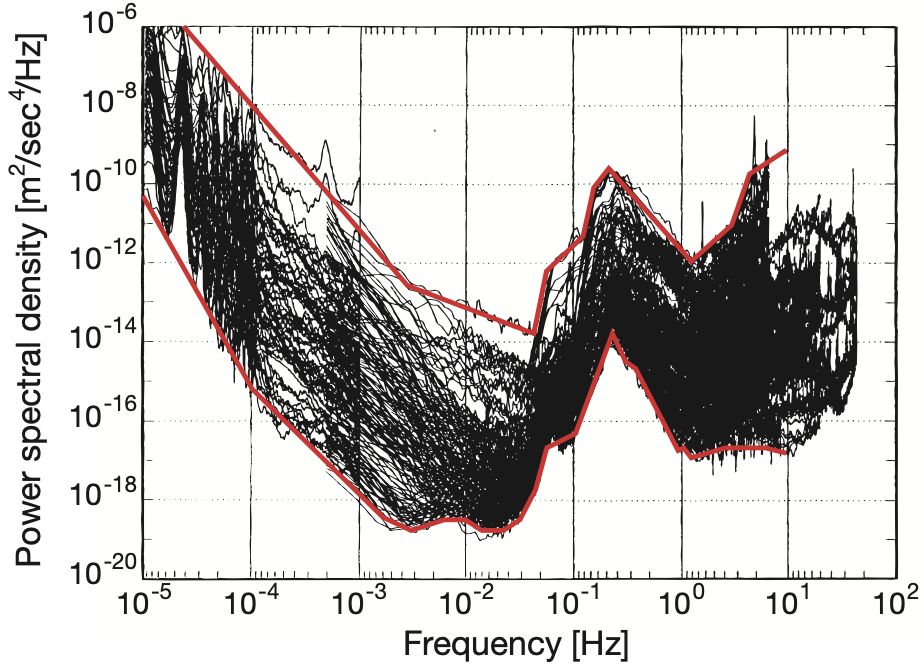
\includegraphics[width=100mm]{fig2_11.png}
\caption[NHNM/NLNMと世界中の地面振動のスペクトル]{NHNM/NLNM(赤い線がそれらを示す)と世界中の地面振動のスペクトル\cite{33}}
\label{fig2.11}
\end{center}
\end{figure}
地面振動雑音の性質は, J. Petersonによって研究されている\cite{33}. 彼は世界中の地震計のネットワークから得られた地面振動雑音スペクトルのカタログを作成した. このデータからNHNM/NLNM (New High/Low Noise Model) と呼ばれる地面振動スペクトルのモデルが構築され, 地面振動の上限と下限を与えている(図\ref{fig2.11}). 
これを見ると1 mHz以下の低周波では地面振動のスペクトルが急激に大きくなっていることがわかる(これは地球の潮汐変動による). しかし, このような低周波の地面振動では検出器のテストマスも共に移動するため, 重力波の観測を妨げることはない. 一方, 0.1$\sim$1 Hz付近にあるピークは海の波が海岸にぶつかることで発生するが, これは検出器にとって安定的な観測運転を妨げる外乱となる. また, 10 Hz以上は検出器の感度が良いため特に関心のある周波数帯である. このような地面振動の影響を低減するためには先に述べたように次の2つの点に注意する必要がある. \\
\quad a)\underline{検出器を静かな場所に建設する}\\
\qquad 図\ref{fig2.12}に示した通り, 地下 (KAGRA site) は地上 (Virgo/TAMA site) に比べて地面振動レベル\\\qquad が1桁から2桁低い. つまり, 地面振動雑音を低減するという観点から見ると, 地下に検出器を建設\\\qquad するのが良いと言える. 
\begin{figure}[H]
\begin{center}
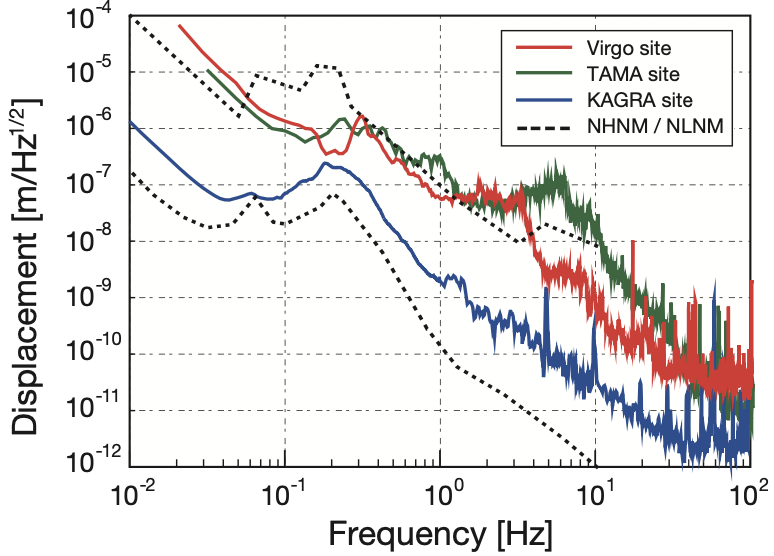
\includegraphics[width=100mm]{fig2_12.png}
\caption[地面振動雑音のスペクトル]{重力波検出器が設置されている場所での地面振動雑音のスペクトル\cite{34}}
\label{fig2.12}
\end{center}
\end{figure}
\noindent
\quad b)\underline{防振系により地面振動を減衰させる}\\
\qquad 防振系によって地面振動を減衰し, 鏡の支点に伝わる振動を小さくする必要がある. \\\qquad 防振系による地面振動の低減については第\ref{第3章}章に詳記する. 

\subsection{世界のレーザー干渉計型重力波検出器}
アメリカのinitial LIGO, イタリア・フランスのVirgo, ドイツのGEO600, 日本のTAMA300といった第1世代重力波検出器と呼ばれる検出器では, FPMIにパワーリサイクリングを組み合わせたものが主流であった. 現在はそれらの検出器に改良を加え, RSEや真空場のスクイージングなどの技術を組み込んだ第2世代重力波検出器が運用されている. また, 更なる感度向上を目指して, 第3世代の重力波検出器を地球上に建設することが計画されている. \\
\quad 以下では世界で用いられている, あるいは計画されている重力波検出器について述べる. 
\subsubsection{現在運用されている重力波検出器}
\vskip3mm
\noindent
\underline{\bm{{\large Advanced LIGO}}}\\
\quad LIGOはアメリカ(リビングストンおよびハンフォード)にある基線長4 kmのレーザー干渉計型重力波検出器である\cite{LIGO}. 2つの観測所は約3000 km離れているため, この2地点における重力波波形の相異性や到達時間の差などから, 重力波信号の真偽の判定が, ある程度できるように考慮されている. . 1990年代から重力波検出の研究を牽引してきたLIGOは, 感度向上を目指してRSEや125 Wのハイパワーレーザー, 4段の鏡懸架系などの技術を導入した後, Advanced LIGOとして観測を開始し, 2015年9月14日, 世界で初めて重力波を検出した. その後も感度向上を目指した改修作業を続け, 数多くの重力波イベントを観測している. \\\\
\underline{\bm{{\large Advanced Virgo}}}\\
\quad Virgoはイタリア(ピサ)にある基線長3 kmのレーザー干渉計型重力波検出器である\cite{Virgo}. 当初からアウトプットモードクリーナーやSuper Attenuator\cite{Virgo}と呼ばれる多段懸架系を導入していたVirgoでも, LIGOと同様の改良が行われた. そして2017年8月, Advanced VirgoとしてLIGOと共に史上4例目となる重力波検出を達成した. \\\\
\underline{\bm{{\large GEO600}}}\\
\quad ドイツ(ハノーヴァ)にある基線長600 mのレーザー干渉計型重力波検出器である\cite{GEO}. GEO600には腕共振器はないが, マイケルソン干渉計にパワーリサイクリング・シグナルリサイクリングを併用しており, 特定の周波数帯域で高感度を実現した. その後, Advanced LIGOなどとの高周波での相関検出を目指して改修され, 現在は1 kHz以上での周波数で感度を高めている. \\\\
\underline{\bm{{\large KAGRA}}}\\
\quad 日本(岐阜県飛騨市神岡町)にある基線長3 kmのレーザー干渉計型重力波検出器である\cite{KAGRA}. KAGRAでは熱雑音低減のためサファイア製の鏡を20 Kまで冷やし, かつ地面振動の影響を減らすために地下環境で運用するという特徴を持つ. 地面振動については第3章, KAGRAの干渉計のレイアウトや懸架系および冷却システムについては第3, 4章を参照されたい. 
\subsubsection{計画中の重力波検出器}
\vskip3mm
\noindent
\underline{\bm{{\large LIGO-India}}}\\
\quad LIGO-IndiaはAdvanced LIGOの部品を一式インドに送り, アメリカとインドの共同でAdvanced LIGOに相当する重力波検出器をインドに建設しようという計画である. LIGO-Indiaの完成により6台の干渉計による国際ネットワークが構築され, 波源の位置特定精度の更なる向上などが見込まれる.\\\\
\underline{\bm{{\large Cosmic ExplolerとEinstein Telescope}}}\\
\quad Cosmic ExplolerとEinstein Telescopeはどちらも将来建設が予定されている第3世代の地上重力波検出器である. Cosmic ExplolerではL字型で1辺40 kmの基線長\cite{31}, Einstein Telescopeでは1辺10 kmの正三角形にすることが予定されている\cite{32}. また, 腕の長さを伸ばしたり, 低吸収のコーティングや周波数依存スクイージングなどの技術を活用することも計画されている. 特に, 低温かつ地下環境での運転が予定されているETでは, KAGRAで培われた運用技術が応用可能であることが期待される. \\
\quad これらの新しい検出器は感度を今よりも10倍以上改善することを目指している. ここで, 重力波検出器の感度は検出可能な波源までの距離に反比例する. つまり感度が10倍良くなれば, 10倍の距離, 検出頻度(体積)で言うと1000倍に膨れ上がることになる. \\
\quad 次世代の検出器ではこのような大幅な感度向上によって, 現在の検出器では叶わないサイエンス(例えば2.1.4.2で述べたパルサーの軸対称からのずれは非常に小さく, 現在運転中の重力波検出器ではパルサーからの重力波を捉えることはできない可能性がある. 他にも, あらゆる天体に対して物理学的なモデルを確定させるためには様々な質量・スピンを持った相当数の重力波信号が必要であることを考えると, 現在の検出器では検出数が不十分である恐れがある. )を達成するという目的がある. 